\def\newcite#1{\cite{#1}}

\def\noun{\textsc{N}}
\def\verb{\textsc{V}}
\def\sg{\textsc{Sg}}
\def\pl{\textsc{Pl}}
\def\detdef{\textsc{DetDef}}


\chapter{Analysing Constraint Grammar}
\label{chapterCGana}

\epigraph{\it Another desirable facility in the grammar development
  environment would be a mechanism for identifying pairs of rules that
  contradict each other.}{Atro Voutilainen, 2004}

In the previous chapter, we presented a tool.
In the current chapter, we will solve a problem.


Recall the design principles of CG from Section~\ref{sec:properties}: 
by design, the grammars are shallow and low-level.
There is no particular hierarchy between lexical, morphological,
syntactic or even semantic tags: individual rules can be written to address any
property, such as ``verb'', ``auxiliary verb in first person singular'',
or ``the word form \emph{sailor}, preceded by \emph{drunken} anywhere in the
sentence''. This makes it possible to treat very particular edge
cases without touching the more general rule: we would simply write
the narrow rule first (``if noun AND \emph{sailor}''), and introduce
the general rule (``if noun'') later.


However, this design is not without problems. As CGs grow larger, it
gets harder to keep track of all the rules and their interaction.
Despite this well-known issue, there has not been a tool that would help 
grammar writers to detect conflicting rules.
Following the idea further, the tool could give feedback that is not 
restricted to conflicts, but also other features that are helpful 
in the process of writing grammar.
Given the rules in Figure~\ref{fig:infrules}, a grammar writer may 
ask the following questions.



\begin{itemize}
\item Are all the Portuguese rules distinct? (e.g. \texttt{Para} and \texttt{De} may be included in \texttt{Prep})
\item Could two or more rules be merged? (e.g. \texttt{SELECT Inf IF -1 Prep OR Vai OR Vbmod ...})
\item What is the best order for the rules?
\item Can the Finnish rule on the left be rewritten in the form shown on the right?
\item Generate an example sequence that triggers rule(s) $R$ but not rule(s) $R'$. 
\end{itemize}

%%%%%


\begin{figure}[t]
\ttfamily
\centering
\begin{tabular}{l | @{~~~} l  l}
SELECT Inf IF ... & \multicolumn{2}{c}{SELECT V + Prs/Imprt + Act + Neg IF ...} \\
~~(-1 Prep) (0C V) ;       & (*-1C Negv LINK NOT *1 Vfin)  & (NOT *-1 Niin OR Neg)  \\
~~(-1 Para OR De) (0C V) ; & (NOT 0 N) (NOT 0 Pron)        & (*-1C Negv \\
~~(-1C Vbmod) (0C V) ;     & (NOT *1 Neg) (NOT *-1 Neg)    &  ~~LINK NOT 0 Imprt \\
~~(-1C Vai) ;              & (NOT 0 Pass) (NOT *-1 Niin)   &  ~~LINK NOT *1 Vfin OR CLB?) \\
~~(-1C Vbmod) (0 Ser) ;    & (*-1C Negv LINK NOT *1 CLB?)  & (NOT 0 N OR Pron OR Pass) \\
~~(-1C Ter/de) ;           & (*-1C Negv LINK NOT 0 Imprt) ;  & (NOT *1 Neg) ; \\

\end{tabular}

\caption{Left: rules to select infinitive in Portuguese. 
        Right: two versions of a condition in Finnish.}

\label{fig:infrules}
\end{figure}

The chapter follows with introduction of related work: namely,
corpus-based methods to aid grammar writing, and automatic
optimisation of a complete, human-written grammar. We continue by
presenting our solution, along with a working implementation, and
finally, evaluate its performance.

We include also two later developments. Section~\ref{sec:basqueEval},
based on the article ``Cleaning up the Basque grammar: a work in
progress'' \cite{listenmaa2017basque}, describes a practical
application of our tool and collaboration with CG writers.
Section~\ref{sec:expressivity} presents the main ideas from
``Exploring the Expressivity of Constraint Grammar''
\cite{kokke2017expressivity}---a side effect following the creation of
\emph{symbolic sentences}, it allowed us to pose the question ``what
if CG was a generative formalism?''

\section{Related work}
\label{sec:CGanaRelated}

There has been previous research on corpus-based methods in manual
grammar development \cite{voutilainen2004}, as well as optimisation of
hand-written CGs~\cite{bick2013tuning}.  In addition, there is a large
body of research on automatically inducing rules,
e.g. \cite{inducing_cg1996,lindberg_eineborg98ilp,lager01transformation,asfrent14}.
However, since our work is aimed to aid the process of hand-crafting
rules, we omit those works from our discussion. Due to adding
Section~\ref{sec:expressivity}, we also include work addressing the
  expressivity and complexity of CG.


\paragraph{Corpus-based methods in manual grammar development}

Hand-annotated corpora are commonly used in the development of CGs, because they give immediate feedback whether a new rule increases or decreases accuracy.
% This helps the grammar writer to arrange the rules in appropriate sections, with safest and most effective rules coming first.
% However, this method will not notice a missed opportunity or a grammar-internal conflict, nor suggest ways to improve.
Atro Voutilainen \cite{voutilainen2004} gives a detailed account about best practices of grammar writing and efficient use of corpora to aid the grammar development.
For a language with no free or tagset-compatible corpus available, Reynolds and Tyers \cite{tyers_reynolds2015} describe a method where they apply their rules to unannotated Wikipedia texts and pick 100 examples at random for manual check.

CG rules are usually arranged in sections, and run in the following manner. 
First apply rules from section 1, and repeat until nothing changes in the text. Then apply rules from sections 1--2, then 1--3 and so on, until the set includes all rules.
The best strategy is to place the safest and most effective rules in the first sections,
so that they make way for the following, more heuristic and less safe rules to act on.
A representative corpus is arguably the best way to get concrete numbers---how many times a rule applied and how often it was correct---and to arrange the rules in sections based on that feedback.

Voutilainen \cite{voutilainen2004} states that the around 200 rules are probably enough to resolve 50--75 \% of ambiguities in the corpus used in the development. 
This figure is very much thanks to Zipf's law: we can add rules that target the most frequent \emph{tokens}, thus disambiguating a high number of word forms.
However, this method will not notice a missed opportunity or a grammar-internal conflict, nor suggest ways to improve; neither does it guarantee a coherent whole of rules. 
While the coverage information is easy to obtain from a corpus, there is no tool that would aid grammar writers in including wide coverage of different linguistic phenomena.


\paragraph{Automatic optimisation of hand-written grammars }

The corpus-based method can tell the effect of each single rule at their place in the rule sequence, and leaves the grammar writer to make changes in the grammar.
As a step further, Eckhard Bick \cite{bick2013tuning} modifies the grammar automatically, by trying
out different rule orders and altering the contexts of the rules. 
Bick reports error reduction of 7--15\% compared to the original grammars.
This is a valuable tool, especially for grammars that are so big that it's hard to keep track manually. A program can try all combinations whereas trying to make sense out of a huge set of rules would be hard for humans.
As a downside, the grammar writer will likely not know why exactly does the tuned grammar perform better.


\paragraph{Expressivity and complexity of CG}
Tapanainen \cite{tapanainen1999phd} gives an account of the expressivity of
the contextual tests for 4 different constraint formalisms, including CG. 
In addition, parsing complexity can be easily defined for a given variant and 
implementation of CG; see for instance Nemeskey \cite{nemeskey14}.
Yli-Jyrä \cite{ylijyra2017} relates CG to early formal language theory, and
provides an independent proof of non-monotonic\footnote{A monotonic
  variant of CG may only remove readings from cohorts, whereas a non-monotonic
  variant may add readings or cohorts.} CG being Turing-complete.

\section{Analysing CGs}
\label{sec:sectionCGana}

We start by defining a conflict, and present requirements for a solution.
Then, we introduce a logical translation of sequential CG, corresponding to \cite{lager_nivre01}, and modify it into a SAT-problem about the \emph{original} sentence before applying the rules.
%this will tell us if it is possible for a senten
We refine our solution by restricting what kind of sentences we can create.
The whole method requires only a morphological lexicon, no corpus. 

\paragraph{Conflict}

We define \emph{conflict} as follows: a list of rules $R$ is in conflict with the rule $r$, if applying $R$ makes it impossible to apply $r$, regardless of input. 
Some examples of conflicts follow:

\begin{itemize}
\item If two equivalent rules $r$ and $r'$ occur in the grammar, the second occurrence will be disabled by the first
\item A list of rules $R$ selects something in a context, and $r'$ removes it
\item A list of rules $R$ removes something in a context, and $r'$ selects it
\item A list of rules $R$ removes something from the context of a rule $r'$, so $r'$ can never apply
\item A rule $r$ has an internal conflict, such as non-existent
tag combination, or contradictory requirements for a context word
\end{itemize}

This definition is very similar to the concept \emph{bleeding order} in generative phonology \cite{kiparsky1968}; however, since we are talking about an explicit list of 
human-written rules, we include also rule-internal conflicts in our classification.
The conflicting (or ``bleeding'') $R$ can be a single rule or a list of rules: for instance, if one rule removes a verb in
context $C$, and another in context $\neg C$, together these rules
remove a verb in all possible cases, disabling any future rule that
targets verbs.

% While rule-internal conflicts can be detected by simpler means, taking
% care of rule interaction requires a {\em semantic} rather than a {\em
%  syntactic} analysis.
% In order to find effects of rule interaction, we must keep track of
% the possible sentences at each step. After each rule, we have two
% possibilities: the rule fires, or it does not fire. In case the rule does
% not fire, we have again two options: either its conditions are not met,
% or its target is the only remaining analysis. 

\paragraph{Solution}

How do we find out if a rule $r$ can act? 
We could apply the grammar to a large corpus and count the number of times 
each rule fires; if some rule never fires, we can suspect there is something wrong 
in the rule itself, or in the interaction with previous rules. 
But it can also be that $r$ just targets a rare phenomenon, and there was no sentence in the corpus that would trigger it.

Of course, tagged corpora are extremely useful for many questions in CG analysis.
A corpus can show which rules are the most used, or which rules give false analyses. 
Luckily, we have already methods for finding such statistics---the question 
about conflicts is orthogonal to those, and the solution needs to address only 
the part about conflicts, not about rules being frequent or accurate.
Therefore, we can take a more artificial approach. % generate our own sentences.
Remember the definition of conflict: ``applying $R$ makes it impossible to apply $r$ \emph{regardless of input}''.
In a nutshell, we are going to show the absence of a conflict by trying to create 
a sequence where $r$ can apply after $R$; conversely, we detect a conflict by 
showing that such sequence cannot be created.



%%%%%%%%%%%%%%%%%%%%%%%%%%%%%%%%%%%%%%%%%%%%%

\def\newVar{$\text{\em word}'_\textsc{ RD}$}
\def\oldVar{$\text{\em word}_\textsc{\,RD}$}
\def\eqdef{\Coloneqq}
\def\invConds{\text{invalid condition}}
\def\onlyTrgLeft{\text{only target left}}

\subsection{From disambiguation to generation}

\paragraph{SAT-encoding of sequential CG}
\label{sec:orderedScheme}

In order to analyse real-life CGs, we need to model the semantics of sequential CG: 
rule application takes effect immediately, is irreversible\footnote{As pointed out by Eckhard Bick, VISL CG-3 allows reference to deleted readings. In principle, this would not be an obstacle for our implementation, because no variables are removed.}, and only allows changes in the target.
We restrict ourselves to the operations on morphological disambiguation, and only {\sc select} and {\sc remove} rules. 
The following encoding does not support dependency relations, nor rule types which add readings or cohorts. 
%In order to support the full feature set of  most likely, we will have to modify our encoding to fully support the features of VISL CG-3.

%There is no way around it: an analysis that treats \t{REMOVE~v ; REMOVE~v~IF~(-1~det)} the same as \t{REMOVE~v~IF~(-1~det) ; REMOVE~v} is worth nothing. The first one is a true conflict, because the first rule has a broader condition; it removes the verb in any possible case. The second rule order is possible: there can always be a sentence that has a verb, but is not preceded by a determiner, hence the first rule would not match, and the verb is saved for the second rule. 
%
%
%
%We need to model the state of the sentence after each rule application. 
%Luckily, we do not need to reinvent the wheel\footnote{of course we did. like, who reads other people's papers.}: 
% This is done in \cite{lager_nivre01}: they present CG as a composition of predicates, 
% numbered by the rules in the grammar. Each predicate is applied to the result of the previous 
% applications, and the ``do not remove last reading'' property is checked each time.
%
%
Last time, we only used ordering as a way to choose the which rules to apply.
But there was no state: all clauses operated in parallel, on the same variables. 
Now, we need a new variable for a reading every time when it is targeted; 
that is, when its state potentially changes.
%But now, we assume that each variable starts off as true: 
%all those readings are true at the ``first round'', and the goal is to make more and more readings false, as more rules are applied.
As before, a sentence is a vector of cohorts, which is, in turn, a vector of variables representing the readings of the current cohort.
At each rule application, we create a new variable \newVar{} for each targeted reading \oldVar{}.
The new variable \newVar{} is true iff 

\begin{figure}[h]
\begin{tabular}{l l}
(a) \oldVar{} was true, and 
                             & (b) the rule cannot apply: this can be because \\
                                     & ~~~~-- its conditions do not hold, or \\
                                     & ~~~~-- it would remove the last reading.
\end{tabular}
\end{figure}

\noindent We keep the same example sequence from Chapter~\ref{chapterCGSAT}, {\em la casa grande}. In the following, we apply the rule \t{REMOVE v IF (-1 det)} to it.

$$\begin{array}{r l}
\text{New variable } \casa{}'_\v 
      & \Longleftrightarrow \quad \casaV\ 
        \wedge\: ( \; \ob{\neg\laDet}^{\invConds} 
        \vee  \ob{(\casaV \wedge \neg \casaN) }^{\onlyTrgLeft} ) \\
\end{array}$$


\noindent After the application, we replace each \oldVar with \newVar in the sentence vector; those variables that are not touched by the rule, will be carried over to the next round unchanged. 
For example, if we apply two rules which target verbs and one which targets pronouns, 
the sentence vector will look like the following. 


%\begin{figure}
$$\begin{array}{r @{~\rightarrow~} l}
\emph{la} & \{\laDet, \la{}'_\prn \} \\
\emph{casa} & \{\casa{}''_\v, \casaN \} \\
\emph{grande} & \{ \grandeAdj \} \\
\end{array}$$
%\label{fig:after3Rules}
%\end{figure}


\paragraph{Symbolic sentence}

We saw how $\casa{}'_\v$ was created, based on the status of $\casaV$ and the conditions at the time. Similarly, $\casa{}''_\v$ will be created based on $\casa{}'_\v$. 
%If there is a pronoun in its conditions, and the rule which targest
But what is the status of the variables in the beginning?
%We have not specified yet what is the status of the variables in the beginning. 
In fact, that decision makes a crucial difference. 
If all variables start off as true, then we have, in effect, reimplemented the logical encoding by Lager and Nivre \cite{lager_nivre01}. 
This option would not make an interesting SAT-problem: 
there is no search involved, just manipulation of Boolean expressions in a completely deterministic way.
All the new variables, created from the rule applications, would get their value immediately: $\casa{}'_\v \Leftrightarrow \grandeAdj \wedge \neg (\casaV \wedge \neg \casaN)$ just translates into $\casa{}'_\v \Leftrightarrow \text{\em True} \wedge \neg (\text{\em True} \wedge \neg \text{\em True})$. 

%There is nothing to decide, no search whatsoever; this problem is even simpler than the animal problem, where we at least had some choices to make.


%However, when all the readings start off as unassigned, the SAT-problem becomes 
%``Which readings were true before any rule applications?''
In order to turn this problem into a SAT-problem, we will have the readings start off
unassigned. All the other variables computed along the way depend on the original variables, so the question to the SAT-solver becomes: \emph{``Which readings were originally true?''}
For implementing a CG engine, this question does not make much sense: we know which readings were given by the morphological analyser. 
But our task now is to {\em generate} the original sentence, which will pass through the rules. 
Here comes the most important modification: we will apply the rules to something we call {\em symbolic sentence}. 
Every cohort, called {\em symbolic word}, contains every possible reading, and rule applications are responsible for shaping the sentence into a concrete one.

% Our analysis operates on a rule $r$, which is preceded by a list of rules $R$, and is concerned with answering the following question: ``Does there exist an input sentence $S$ that can trigger rule $r$, even after passing all rules $R$ that came before $r$?''
% Instead of concrete sentences from a corpus, we apply rules on {\em symbolic sentences}

Before we can do any analysis any of the rules, we need to find out
what the set of all possible readings of a word is. We can do this by
extracting this information from a lexicon, but there are other ways
too; we will explain this in more detail in
Section~\ref{sec:realistic_language}. In our experiments, the number
of readings has ranged from about 300 to about 9000.

\paragraph{Width of a rule}
Furthermore, when we analyse a rule $r$, we need to decide the {\em width} $w(r)$ of the rule $r$: How many different words should there be in a sentence that can trigger $r$? Most often, $w(r)$ can be easily determined by looking at how far away the rule context indexes in the sentence relative to the target. For example, in the rule \t{REMOVE v IF (-1 det)}, the width is 2.

If the context contains a \t{*} (context word can be anywhere),
we need to make an approximation of $w(r)$, which may result in false positives or negatives later on in the analysis; this indeed happened in the Finnish grammar in Section~\ref{sec:finnishEval}. %For the implementation, we tried for each \t{*} multiple variants of the sentence. 
For example, given the rule \t{REMOVE~v~IF~(-1*~det)}, 
we tried first a sentence of width 2; if there was a conflict, we tried width 3, and then 4. For a rule with multiple \t{*}s, we create combinations in the range of $\pm$ 2 symbolic words for each \t{*}-condition; 
in addition, we need to specify where the target is in the symbolic sentence. 
For instance, the rule \t{REMOVE~v~IF~(-1*~det)~(1*~det)} would be tested 
with the following combinations, where C means condition and T means target:
% in a range of 3--7 symbolic words: both \t{1*} and \t{-1*} can be interpreted as \t{}. 
% For the rule with two \t{*}s, we tried all the following combinations: 
(C,T,C); 
(C,C,T,C); 
(C,T,C,C); 
(C,C,T,C,C); 
(C,C,C,T,C,C); 
(C,C,T,C,C,C) and
(C,C,C,T,C,C,C).


%we create sentences that are up to 3 words wider than the context without \t{*}, and try them all.

\paragraph{Rule application}
Finally, we define what does it mean for a sentence to ``pass through'' a rule. 
Let us enumerate the cases:
\begin{enumerate}
\item The sentence is out of scope; target not removed
\item The conditions of the rule do not hold; target not removed
\item The target is the only possible reading left; target not removed
\item The target was never in place
\item The target is removed
\end{enumerate}
%In a symbolic sentence, we cannot properly distinguish between the last two cases. 
Let us illustrate the difference between the last two cases with a rule that targets pronouns, say, \t{REMOVE prn IF (1 v)}. 
If the target was never in place, then both the original $\laPrn$ and the newly created $\la{}'_\prn$ end up as false. 
If the target is removed, then $\laPrn$ will be true and $\la{}'_\prn$ false.
This means that a rule with the condition \t{IF (-1 prn)} behaves differently depending on where in the rule sequence it is placed: 
if it is applied before \t{REMOVE prn IF (1 v)}, then it will match the original reading $\laPrn$. Any rule applied after that will get the newly created variable $\la{}'_\prn$.

%that is, whether the new variable depends on $\laPrn$ or  $\la{}'_\prn$.
%The difference between the last two cases is that, say we have the readings $\laPrn$ and $\la{}'_\prn$

Now we have the definitions in place. In the following, we are going to show two examples; first one a very simple conflict, and the second one with more complicated interaction.


\paragraph{Example 1: conflict}

Let us look at a conflicting case. For simplicity, we assume that the full set of readings in the language is $\{ \emph{det def, noun sg, noun pl, verb sg, verb pl} \}$. We ignore all lexical readings for now, and assume dummy words of the form \emph{w$_{i}$}, where $i$ refers to the index of the word.
The rules are as follows:


\begin{verbatim}
r1 = REMOVE verb IF (-1 det) ;
r2 = REMOVE verb IF (-1 det) (1 noun) ;
\end{verbatim}


We want to know if the last rule is able to apply, after going through the rules that come before it---in this case, there is only one such rule. 
The width of the last rule is three: one condition to the left of the target, one to the right, so we create a symbolic sentence of three words. Below, we show the symbolic sentence, consisting of the symbolic words {\em w1, w2} and {\em w3}.

\begin{figure}[h]
\centering
\begin{tabular}{p{0.6cm} l  p{0.6cm} l p{0.6cm} l }
\t{"<w1>"}    &                     &  \t{"<w2>"}  &           &  \t{"<w3>"}    \\
              & \t{"w1" det def}    & &      \t{"w2" det def}  & &  \t{"w3" det def} \\
              & \t{"w1" noun sg}    & &      \t{"w2" noun sg}  & &  \t{"w3" noun sg} \\
              & \t{"w1" noun pl}    & &      \t{"w2" noun pl}  & &  \t{"w3" noun pl} \\
              & \t{"w1" verb sg}    & &      \t{"w2" verb sg}  & &  \t{"w3" verb sg} \\
              & \t{"w1" verb pl}    & &      \t{"w2" verb pl}  & &  \t{"w3" verb pl} \\
\end{tabular}
\end{figure}

After applying the first rule, we have a situation which looks much like the one in the previous chapter, Figure~\ref{fig:modelsOneRule}. 
If the symbolic word {\em w1} is a determiner, then {\em w2} cannot be a verb; 
the only exception is the case where verb is the only analysis of {\em w2}. 
As before, the verb analysis {\em w2} can also be false, even if {\em w1} 
is not a determiner. The exact same dependencies are created between the 
symbolic words {\em w2} and {\em w3}.
The first word {\em w1} is out of scope of the condition, because it has no preceding word. 
Below we see the affected readings after the first rule application, with newly created variables:

\begin{figure}[h]
$$\begin{array}{l @{~\rightarrow~} l}
1 & \{w1_{\detdef}, \  w1_{\noun\sg}, \  w1_{\noun\pl}, \ w1_{\verb\sg}, \ w1_{\verb\pl} \} \\
2 & \{w2_{\detdef}, \  w2_{\noun\sg}, \  w2_{\noun\pl}, \ w2'_{\verb\sg}, \ w2'_{\verb\pl} \} \\
3 & \{w3_{\detdef}, \  w3_{\noun\sg}, \  w3_{\noun\pl}, \ w3'_{\verb\sg}, \ w3'_{\verb\pl} \} \\
\end{array}$$
\end{figure}

There is no ``final sentence'' yet, simply constraints on the possible combinations of determiners and verbs. If we asked for a solution now, it could be anything; for instance, all three words are determiners. Just asking for a freely chosen sequence is not very interesting; there are so many possibilities, and even after applying more rules, most of the combinations are not explicitly prohibited. 

We want to know if there is a sequence that can trigger the last rule.
In order to trigger the rule, the sequence must have the following three features:
\begin{itemize}
\item Target readings: at least one reading with a \emph{verb} tag in the target position {\em w2}.
\item Ambiguity: at least one reading without a \emph{verb} tag in the target position; if there are only \emph{verb} readings in the target, the rule would not fire.
\item Conditions: at least one reading with a \emph{det} tag in the cohort preceding the target, and at least one reading with a \emph{noun} tag in the cohort following the target.
\end{itemize}


We can see that some of these requirements can be fulfilled: the first rule allows models where {\em w2} contains \emph{target readings}. If the rule had been \t{REMOVE verb}, that is, unconditionally remove all verbs, then this requirement could not be fulfilled. But so far we have not run into the wall. 
The second requirement, for \emph{ambiguity} is no problem either: other readings of {\em w2} have not been targeted, so we are free to choose anything.

As for \emph{conditions}, the part about \t{(1 noun)} can be fulfilled; nothing prevents {\em w3} from being a noun. But the first condition, \t{(-1 det)}, cannot be true, if the target {\em w2} has to be a verb---the first rule has prohibited exactly that combination.
Therefore, when we try to ask for a solution where all these requirements hold, we will get a conflict. The result shows us that the rule \t{REMOVE~verb~IF~(-1~det)~(1~noun)} cannot ever apply, if the rule \t{REMOVE~verb~IF~(-1~det)} has been already applied. 
%For any pair of two rules \t{REMOVE x IF C1} and \t{REMOVE x IF C2}, if $C2 \subseteq C1$, then the latter rule will not have a chance to apply; simply because there is no condition that would fulfil C2 but not C1.
% As we see later from the evaluation, recognising such pairs is not always easy.

\paragraph{Example 2: no conflict}
The previous was a simple example of a conflict: two rules target the same reading, and the first one had broader conditions. 
%and the conditions were chosen such that the first rule applies in more cases than the second.
Since we had only one preceding rule, we could not demonstrate why is it important to apply all the rules in order---even with a longer list of rules, the previous example could have also worked unordered, as long as the last rule is separated from rules before it.
%two rules had the same target, and the first mentioned had a broader set of conditions.
%Furthermore, the order was not really crucial. 
Now we will show another example, where we illustrate why is it important to create new variables, and how conditions can affect the state of the variables, but in a more limited way. The set of readings is the same, and the rules are as follows.

\begin{itemize}
\item[] 
\begin{verbatim}
r1 = REMOVE verb IF (-1C det) ;
r2 = SELECT det  IF ( 1 verb) ;
r3 = REMOVE verb IF (-1 det) ;
\end{verbatim}
\end{itemize}

\noindent The width of the last rule is 2, thus we create a symbolic sentence with only {\em w1} and {\em w2}. The sentence is shown below:

\begin{figure}[h]
\begin{tabular}{p{0.2cm} p{0.6cm} l  p{0.6cm} l }
& \t{"<w1>"}    &                     &  \t{"<w2>"}  &           \\
&              & \t{"w1" det def}    & &      \t{"w2" det def}  \\
&              & \t{"w1" noun sg}    & &      \t{"w2" noun sg}  \\
&              & \t{"w1" noun pl}    & &      \t{"w2" noun pl}  \\
&              & \t{"w1" verb sg}    & &      \t{"w2" verb sg}  \\
&              & \t{"w1" verb pl}    & &      \t{"w2" verb pl}  \\
\end{tabular}
% \label{fig:ambiguousDet}
% \caption{After $r1$, the symbolic word {\em w1} has to be determiner, but ambiguously so.}
\end{figure}


To begin, let us only look at {\em r1} and {\em r3}. Like in the previous example, they target the same reading, but now the order is good: the first rule is the one with a narrower condition, which means that it is possible for a sequence to pass through it, and still have the verb reading in {\em w2} intact---it just needs to have something else in addition to the determiner in {\em w1}.
The following is an example of such sequence (false readings not shown). %---if we stopped after $r1$ and asked for a solution that triggers $r3$, we might get just that.

\begin{figure}[h]
\begin{tabular}{p{0.2cm} p{0.6cm} l  p{0.6cm} l }
& \t{"<w1>"}    &                     &  \t{"<w2>"}  &           \\
&              & \t{"w1" det def}    & &      \t{"w2" noun pl}  \\
&              & \t{"w1" noun sg}    & &      \t{"w2" verb sg}  \\
\end{tabular}
% \label{fig:ambiguousDet}
% \caption{After $r1$, the symbolic word {\em w1} has to be determiner, but ambiguously so.}
\end{figure}


So far, we have passed through {\em r1} with the case ``condition does not hold, target not removed''. Now, let us add {\em r2}: \t{SELECT det IF (1 verb)}. 
We must, in fact, select the determiner and remove everything else: 
the condition of {\em r2} happens to be the target of {\em r3}, so it must hold. 
%if the condition of $r2$ did not hold, then $r3$ would not have its target.
But we have the notion of state now, so this is no problem.
On arriving to {\em r1}, the symbolic word {\em w1} had to be ambiguous---that is, one of the variables $w1_{\noun\sg}, \  w1_{\noun\pl}, \ w1_{\verb\sg}, \ w1_{\verb\pl}$ must be true. 
But after passing through {\em r2}, the state of {\em w1} has changed:
it contains a set of new variables $w1'_{\noun\sg}, \ w1'_{\noun\pl}, \ w1'_{\verb\sg}, \ w1'_{\verb\pl}$, and all of them must be false.
Since the clauses formed by {\em r1} and {\em r3} get access to different variables, there is no conflict.

% Thanks to the distinction, the initial {\em w1}, with the primeless variables, does not trigger {\em r1}. 
% The {\em w1} changed by {\em r2} is not visible to {\em r1}, so 
% We have arrived to the situation where {\em w1} at time {\em t1} does not trigger {\em r1}, 
% but {\em w1} at time {\em t3} triggers {\em r3}.


% The state of a given variable can still be affected by a condition, but in a more restricted way.
% We allow \t{w1<n>} to be true and \t{w1'<n>} be false; both true; both false, but not \t{w1<n>} to be false and \t{w1'<n>} true. In other words, a reading may be in place all the time; absent all the time; or in place earlier and get removed later. No other changes are allowed.




% In the system of interconnected clauses, application of rule number 100 may not only affect the target of rule number 1, but conditions as well. 
% A reading may be removed from a symbolic word between rules 1 and 100, if there is a rule that targets it among r2--r99. But if r1 requires w1 to be a noun, and r100 requires it to not be noun, this condition of r100 is not enough to make w1 change its nounhood at random.





\subsection{Towards realistic language}
\label{sec:realistic_language}

\paragraph{Creating realistic readings}
\label{sec:realistic_readings}

Earlier we have shown an example with 5 readings (``det def'', ``noun
sg'', ...). In a realistic case, we operate between hundreds and
thousands of possible readings.  In order to find the set of readings,
we expand a morphological lexicon\footnote{We used the lexica from
 Apertium, found in \url{https://github.com/apertium/apertium-languages}.}, 
ignore the word forms and lemmas, and take all distinct analyses.
However, many grammar rules target a specific lemma or word form.  A
simple solution is to retain the lemmas and word forms only for those
entries where it is specified in the grammar, and otherwise leave them
out. For example, the Dutch grammar contains the following rule:

\begin{itemize}
 \item[] \texttt{REMOVE ("zijn" vbser) IF (-1 Prep) (1 Noun) ;}
\end{itemize}

\noindent This hints that there is something special about the verb
\emph{zijn}, compared to the other verbs. Looking at the lexicon, we
find \emph{zijn} in the following entries:

\begin{itemize}
 \item[] 
\begin{verbatim}
zijn:zijn<det><pos><mfn><pl>     zijn:zijn<vbser><inf>
zijn:zijn<det><pos><mfn><sg>     zijn:zijn<vbser><pres><pl>
\end{verbatim}
\end{itemize}

\noindent Thus we add special entries for these: in addition to the anonymous
``det pos mfn pl'' reading, we add ``\emph{zijn} det pos mfn pl''. 
The lemma is treated as just another tag.

However, for languages with more readings, this approach is not
feasible. For instance, Spanish has a high number of readings, not
only because of many inflectional forms, but because it is possible to
add 1--2 clitics to the verb forms.  The number of verb readings
without clitics is 213, and with clitics 1572.  With the previously
mentioned approach, we would have to duplicate 1572 entries for each
verb. We experimented with small variations with Spanish, and
report slightly different results (and significantly different running
time) in Section~\ref{sec:eval}. Later on, when we applied the tool for Basque
\cite{listenmaa2017basque}, we were forced to modify the approach even
further. We explain the changes in Section~\ref{sec:basqueChanges}.

The readings in a grammar can be underspecified: for example, the rule
\texttt{REMOVE (verb sg) IF (-1 det)} gives us ``verb sg'' and ``det''.
%Set and list definitions were unfolded; a rule such as
In contrast, the lexicon only gives us fully specified readings, such
as ``verb pres p2 sg''. We implemented a version where we took
the tag combinations specified in the grammar directly as our
readings, and we could insert them into the symbolic sentences as well.
The shortcut works most of the time, but if we only take the readings
from the grammar and ignore the lexicon, it is possible to
miss some cases: e.g. the rule \texttt{SELECT (pron rel) IF (0 nom)} 
may require ``pron rel nom'' in one reading, but this method only gives
``pron rel'' and ``nom'' separately. 


In addition, we found that the tag lists in the grammars sometimes
contain errors, such as using a nonexistent tag or using a wrong level
in a subreading. If we accept those lists as readings, we will
generate symbolic sentences that are impossible, and not discover
the bug in the grammar.
However, if we are primarily interested in rule interaction, then using
the underspecified readings from the grammar may be an adequate solution.

%In fact, it may even catch interaction conflicts between rules which have an internal conflict


\begin{table}[h]
\centering
\begin{tabular}{ c|c|c|c|c}
             & \t{n nt sg}  & \t{n f pl}  & \t{vblex sep inf} & \t{det pos mfn}  \\ \hline
 uitgaven    & 0        & 1       & 1             & 0    \\ 
 toespraken  & 0        & 1       & 1             & 0    \\ 
 haar        & 1        & 0       & 0             & 1    \\ 
\end{tabular}
\caption{Ambiguity classes}
\label{table:ambclass}
\end{table}

\paragraph{Creating realistic ambiguities}


In the previous section, we have created realistic \emph{readings}, by simply hardcoding legal tag combinations into variables. The next step in creating realistic \emph{ambiguities} is to constrain which readings can go together. For instance, the case of \emph{zijn} shows us that ``determiner or verb'' is a possible ambiguity. In contrast, there is no word form in the lexicon that would be ambiguous between an adjective and a comma, hence we do not want to generate such ambiguity in our symbolic sentences.


We solve the problem by creating \emph{ambiguity classes}: groups of
readings that can be ambiguous with each other.  We represent the
expanded morphological lexicon as a matrix, as seen in
Table~\ref{table:ambclass}: word forms on the rows and analyses on the
columns. Each distinct row forms an ambiguity class. For example, one
class may contain words that are ambiguous between plural feminine
nouns and separable verb infinitives; another contains masculine
plural adjectives and masculine plural past participles.  Then we form
SAT-clauses that allow or prohibit certain combinations. These clauses
will interact with the constraints created from the rules, and the end
result will be closer to real-life sentences.

Our approach is similar to \newcite{cutting_etal92}, who use ambiguity
classes instead of distinct word forms, in order to reduce the number
of parameters in a Hidden Markov Model. They take advantage of the
fact that they don't have to model ``bear'' and ``wish'' as separate
entries, but they can just reduce it to ``word that can be ambiguous
between noun and verb'', and use that as a parameter in their HMM.
%We can do a similar thing by saving a list of words with each ambiguity class. For example, we map the ambiguity class ``feminine plural noun or a separable verb infinitive'' to the list of word forms \{``uitgaven'', ``toespraken''\}, and then, if we generate such reading for our symbolic word, we can give one of these words as an example word.

There are two advantages of restricting the ambiguity within words.
Firstly, we can create more realistic example sentences, which should help the grammar writer.
Secondly, we can possibly detect some more conflicts. Assume that the grammar contains the following rules:

 \begin{itemize}
 \item[] 
\begin{verbatim}
 REMOVE adj IF (-1 aux) ;
 REMOVE pp  IF (-1 aux) ;
 \end{verbatim}
 \end{itemize}

 With our symbolic sentence, these rules will be no problem; to apply the latter, we only need to construct a target that has a realistic ambiguity with a past participle; the adjective will be gone already.
However, it could be that past participles (pp) only ever get confused with adjectives---in that case, the above rules would contradict each other.
 By removing the adjective reading, the first rule selects the past participle reading, making it an instance of ``$r$ selects something in a context, $r'$ removes~it''. 
The additional constraints will prevent the SAT-solver from creating an ambiguity outside the allowed classes, and such a case would be caught as a conflict.

\subsection{Use cases}

In the beginning of this chapter, we gave a list of questions, regarding the rules in Figure~\ref{fig:infrules}. After describing our implementation, we return to these questions, and explain how a SAT-solver can answer them. 
Section~\ref{sec:eval} shows the evaluation of the conflict detection, which we tried out for four grammars of different sizes. 
The use cases presented in this section have not been tried in practice; however, our setup makes them fairly straight-forward to implement.

\paragraph{Are all the rules distinct?} We gave the example of two rules in the Portuguese grammar, where one had the condition \t{(-1 Prep)} and the other \t{(-1 Para OR De)}. A grammarian who has some knowledge of Portuguese could tell that {\em para} and {\em de} are both prepositions, so these two rules seem to do almost the same thing.

How can we verify this? To start, we apply all candidate rules to the same initial symbolic sentence. For the resulting symbolic sentence, we can ask for solutions with certain requirements.
For instance, ``give me a model where a reading $a \notin \t{Inf}$ is true''.
There are less such models allowed after \t{SELECT Inf IF (-1 Prep)}---if 
a non-infinitive reading is in place, it means that the previous word cannot be any determiner---and 
they are all in the set of models allowed \t{SELECT Inf IF (-1 Para OR De)}. Thus, we can show that the first rule implies the second. It is in the hands of the grammar writer to decide whether to keep the stronger or the weaker rule, or if they should be placed in different sections.


\paragraph{Could two or more rules be merged?} This example concerns two or more rules with the same target but different conditions in the same position. 
All the six rules in Figure~\ref{fig:infrules} have conditions in position -1; four of them also in 0. Some of them have an additional careful context, and some do not.
A grammar writer might think that \t{IF (-1C Vbmod) (0C V)} and \t{IF (-1C Vbmod) (0 Ser)} are very similar, and could be merged into \t{SELECT Inf IF (-1C Vbmod) (0C V OR Ser)}. But could there be some unintended side effects in merging these two rules? Why is there a C in the first rule, but not in the second rule? 

The procedure is similar to the previous one. We initialise two symbolic sentences; on one we run the original rules in a sequence, and on the other the merged rule. 
Then, we can perform tests on the resulting symbolic sentences. Assuming that the ambiguity class constraints are in place, the result may show that C is not needed for the condition about {\em ser}, simply because {\em ser} is not ambiguous with anything else in the lexicon; hence the merged rule can safely have the condition \t{(0C V OR Ser)}. However, if {\em ser} can be ambiguous with something else, then this merged rule is stricter than the two original rules. If the grammar writer is still unsure whether there would be any meaningful sequences that would be missed, they can ask the SAT-solver to generate all those cases---this requires that the ambiguity classes are implemented, 
otherwise the number of solutions would blow up due to all the readings that are irrelevant to the rules in question.
%\formulation{otherwise the number of solutions would be exponential on all possible readings in the lexicon.} 

\paragraph{Generate a sequence that triggers rule(s) $R$ but not rule(s) $R'$.}
For any given rule, we can extract three requirements that would make it trigger. We illustrate them for the rule \t{REMOVE v IF (-1 det)}. In order to trigger the rule, the sequence must have
\begin{itemize}
\item target readings: at least one reading with the \emph{v} tag in the target position
\item ambiguity: at least one reading without the \emph{v} tag in the target position; if there are only \emph{v}-readings in the target, the would not fire.
\item conditions: at least one reading with the \emph{det} tag in the cohort preceding the target.
\end{itemize}

We can extract these requirements from both the rules that must be triggered, and the rules that must be not triggered. Then, we can request a solution from the SAT-solver.

\paragraph{What is the best order for the rules?}
We can generate variants of the rule order, and run them to a set of symbolic sentences. Then, for the resulting symbolic sentences, we can query which one is the most restricted, that is, allows the least models.
As a variant, we may be interested in the placement of just one rule in the sequence.

\paragraph{Does a rewritten rule correspond to the original?}
We can initialise two symbolic sentences, then run the original rule and the rewritten rule, and check if they allow the same models. 

\section{Evaluation}
\label{sec:eval}

We tested two grammars with the setup described in
Section~\ref{sec:realistic_language}: readings as combinations of
lexical and morphological tags, and ambiguity class constraints in place.
These grammars were very small:
Dutch\footnote{\scriptsize{\url{https://github.com/apertium/apertium-nld/blob/master/apertium-nld.nld.rlx}, commit d13fdaa}},
with 59 rules and 
Spanish\footnote{\scriptsize{\url{https://github.com/apertium/apertium-spa/blob/master/apertium-spa.spa.rlx}, commit 1d4f290d}},
with 279 rules.

In addition, we applied variations of the method to two grammars,
which were both larger and targeted more complex languages:
Finnish\footnote{\scriptsize{\url{https://github.com/flammie/apertium-fin/blob/master/apertium-fin.fin.rlx}, commit 49866f3b}},
with 1185 rules, and
Basque\footnote{\scriptsize{\url{https://github.com/inariksit/cgclean/blob/master/data/gramatika4.4.1_lem.rlx}, commit 793e00d1}}
with 1261 rules. Due to the size of the grammars and tagsets, we had
to apply some shortcuts; these are described in the relevant sections.

We left out \textsc{map}, \textsc{substitute} and other rule
types introduced in CG-3, and only tested \textsc{remove} and \textsc{select} rules.
The results for Dutch and Spanish are shown in Table~\ref{table:res},
and the results for Finnish in Table~\ref{table:resFin}. For Basque,
we were unable to analyse the whole grammar; instead we worked in
smaller batches. 


The experiments revealed problems in all grammars. For the smaller
grammars, we were able to verify manually that nearly all detected conflicts were
true positives---we found one false positive and one false negative,
when trying out different setups for the Spanish grammar. 
%The results for the Finnish grammar are inconclusive, 
% For the Finnish grammar, we did not have time to
% investigate all of them, but among those we could, we found both true and false negatives.
We did not systematically check for false negatives in any of the
grammars, but we kept track of a number of known tricky cases; mostly
rules with negations and complex set operations.
As the tool matures and we add new features, a more in-depth analysis
will be needed.
Another natural follow-up evaluation will be to compare the accuracy of the
grammar in the original state, and after removing the conflicts found
by our tool. 
%We aim to perform such evaluation, when the toolset is more mature.


\begin{table}[h]
\centering
\begin{tabular}{|p{2.84cm}|p{1cm}|p{1.15cm}|p{1.55cm}|}
%\begin{tabular}{|p{2.9cm}|p{0.95cm}|p{1.15cm}|p{1.55cm}|}

\hline
                   & \textsc{nld}  & \textsc{spa}  & \textsc{spa}~\textsuperscript{sep.~lem.} \\ \hline
\# rules           & 59            & 279       & 279     \\ \hline
\# readings        & 336           & 3905      & 1735    \\ \hline
\# true~positives~\textsuperscript{AC}% with~amb.~classes
                   & 7             & 45        & 44      \\ 
{\small (internal~+~interaction)}
                   & {\small
                      (6~+~1)}     & {\small 
                                    (21~+~24)} & {\small (20~+~24)} \\ \hline

\# true~positives~\textsuperscript{no AC}  & 7             & 43        & 42      \\ 
{\small (internal~+~interaction)}
                   & {\small
                      (6~+~1)}     & {\small 
                                    (18~+~25)} & {\small (17~+~25)} \\ \hline
\# false positives 
                   & 0             & 0        & 1  \\ \hline

\clock{} with amb. 
           classes & 7 s        & 1h 46m   &  23 min  \\ \hline

\clock{} no amb. 
           classes & 3 s        & 44 min       & 16 min     \\ \hline 


\end{tabular}
\caption{Results for Dutch and Spanish grammars.}
\label{table:res}
\end{table}

\subsection{Dutch} The Dutch grammar had two kinds of errors: rule-internal and rule interaction. As for rule-internal conflicts, one was due to a misspelling in the list definition for personal pronouns, which rendered 5 rules ineffective. The other was about subreadings: the genitive \emph{s} is analysed as a subreading in the Apertium morphological lexicon, but it appeared in one rule as the main reading. 
There was one genuine conflict with rule interaction, shown below:

\begin{itemize}
\item[\textsc{d$_1$.}] 
\begin{verbatim}
REMOVE Adv IF (1 N) ;
REMOVE Adv IF (-1 Det) (0 Adj) (1 N) ;
\end{verbatim}
\end{itemize}

% These two rules both remove an adverb, but the first one has a broader condition:
% remove adverb if followed by a noun. In contrast, the second rule has a stricter condition: only remove adverb if it is preceded by a determiner, the adverb itself is ambiguous with an adjective, and followed by a noun. 
\noindent These two rules share a target: both remove an adverb.
The problem is that the first rule has a broader condition than the second, hence the second will not have any chance to act. 
If the rules were in the opposite order, then there would be no problem.



We also tested rules individually, in a way that a grammar writer might use our tool when writing new rules.
The following rule was one of them:

\begin{itemize}
\item[\textsc{d$_2$.}] 
\texttt{SELECT DetPos IF (-1 (vbser pres p3 sg)) (0 "zijn") (1 Noun);}
\end{itemize} 

\noindent As per VISL CG-3, the condition \texttt{(0 "zijn")} does not require
 \emph{zijn} to be in the same reading with the target \t{DetPos}.
It just means that at index 0,
there is a reading with any possessive determiner, and a reading with any \emph{zijn}.
However, the intended action is to select a ``det pos \emph{zijn}'' all in one reading;
this is expressed as \texttt{SELECT DetPos + "zijn"}.
In contrast, the 0-condition in example~\textsc{d$_1$} is used correctly:
the adjective and the adverb are supposed to be in different readings.


Can we catch this imprecise formulation with our tool? The SAT-solver will not mark it as a conflict (which is the correct behaviour). But if we ask it to generate an example sequence, the target word may be either of the following options. Seeing interpretation a) could then direct the grammar writer to modify the rule.

\begin{itemize}
\item[a)] \begin{verbatim}
"<w2>"
    "w2" det pos f sg
    "zijn" vbser inf
\end{verbatim}

\item[b)] \begin{verbatim}
"<w2>"
    "zijn" det pos mfn pl
\end{verbatim}
\end{itemize}


We found the same kind of definition in many other rules and grammars.
To catch them more systematically, we could add a feature that alerts in all cases where a condition with 0 is used. As a possible extension, we could automatically merge the 0-condition into the target reading, then show the user this new version, along with the original, and ask which one was intended.

% In the latter case, the grammar writer would hopefully notice the imprecise definition and change their definition. However, this is more of a happy side effect than intended feature---the grammar writer cannot count on our tool to notice all similar cases.

\subsection{Spanish} The Spanish grammar had proportionately the
highest number of errors. The grammar we ran is like the one
found in the Apertium repository (linked on the previous page), 
apart from two changes: we fixed some typos (capital O for 0) in order to make it compile, and
commented out two rules that used regular expressions, because we did not implement the support for them yet.
For a full list of found conflicts, see the annotated log of running our program in \url{
https://github.com/inariksit/cgsat/blob/master/data/spa/conflicts.log}. 


We include two versions of the Spanish grammar in Table~\ref{table:res}: in column \textsc{spa}, we added the lemmas and word forms as described in Section~\ref{sec:realistic_readings}, and in column \textsc{spa}\textsuperscript{sep.~lem.}, we just added each word form and lemma as individual readings, allowed to combine with any other reading. 
This latter version ran much faster, but failed to detect an internal conflict for one rule, and reported a false positive for another. 
% FAIL TO DETECT: SELECT:pr_cnjadv_3 cnjadv IF (0 "después de") 
% FALSE POSITIVE: SELECT:este_1 det IF (0 "este" + (m sg)|(m sp)|(mf sg)|(mf sp))

When we added ambiguity class constraints, we found three more internal conflicts.
Interestingly, the version with ambiguity classes fails to detect an interaction conflict, which the simpler version reports, because one of the rules is first detected as an internal conflict. 
We think that neither of these versions is a false positive or negative; it is just a matter of priority. Sometimes we prefer to know that the rule cannot apply, given the current lexicon. 
However, we may know that the lexicon is about to be updated, and would rather learn about all potential interaction conflicts.

As an example of internal conflict, there are two rules that use \texttt{SET Cog = (np cog)}: the problem is that the tag ``cog'' does not exist in the lexicon. As another example, four rules require a context word tagged as NP with explicit number, but the lexicon does not indicate any number with NPs. It is likely that this grammar has been written for an earlier version, where such tags have been in place.
One of the conflicts that was only caught by the ambiguity class constraints had the condition \texttt{IF (1 Comma) (..) (1 CnjCoo)}. The additional constraints correctly prevent commas from being ambiguous with anything else.

As for the 25 interaction conflicts, there were only 9 distinct rules that rendered 25 other rules ineffective.
In fact, we can reduce these 9 rules further into 3 different groups: 4~+~4~+~1, where the groups of 4 rules are variants of otherwise identical rule, each with different gender and number.
An example of such conflict is below (gender and number omitted for readability):

\begin{itemize}
\item[\textsc{s$_{1}$.}] 
\begin{verbatim}
# NOM ADJ ADJ
SELECT A OR PP IF (-2 N) (-1 Adj_PP) (0 Adj_PP) (NOT 0 Det);

# NOM ADJ ADJ ADJ
SELECT A OR PP IF (-3 N) (-2 N) (-1 Adj_PP) (0 Adj_PP) (NOT 0 Det);
\end{verbatim}
\end{itemize}


In addition, the grammar contains a number of set definitions that were never
used. Since VISL CG-3 already points out unused sets, we did not add such
feature in our tool. However, we noticed an unexpected benefit when
we tried to use the set definitions from the grammar directly as our
readings: this way, we can discover inconsistencies even in
set definitions that are not used in any rule.
For instance, the following definition requires the word to be all of
the listed parts of speech at the same time---most likely, the grammar writer meant 
OR instead of +:
\begin{itemize}
\item[\textsc{s$_2$.}] 
\texttt{SET NP\_Member = N + A + Det + PreAdv + Adv + Pron ;}
\end{itemize}

If it was used in any rule, that rule would have been marked as
conflicting. We noticed the error by accident, when the program
offered the reading ``\emph{w2}~n~adj~det~preadv~adv~prn''
in an example sequence meant for another rule.


As with the Dutch grammar, we ran the tool on individual rules and
examined the sequences that were generated. None of the following was
marked as a conflict, but looking at the output indicated that there
are multiple interpretations, such as whether two analyses for a
context word should be in the same reading or different readings.
We observed also cases where the grammar writer has specified desired
behaviour in comments, but the rule does not do what the grammar
writer intended. 

\begin{itemize}
\item[\textsc{s$_3$.}] \t{REMOVE Sentar IF (0 Sentar) (..) ;}
\item[] \t{SELECT PP IF (0 "estado") (..) ;}
\end{itemize}

The comments make it clear that the first rule is meant to
disambiguate between \emph{sentar} and \emph{sentir}, but the rule
does not mention anything about \emph{sentir}.  Even with the
ambiguity class constraints, the SAT-solver only created an ambiguity
where \emph{sentar} in 1st person plural is ambiguous with an
anonymous 1st person plural reading.  This does not reflect the
reality, where the target is only ambiguous with certain verbs, and in
certain conjugated forms.

The second case is potentially more dangerous.  The word form
$estado_{W}$ can be either a noun ($estado_{L}$, `state'), or the past
participle of the verb $estar_{L}$.  The condition, however, addresses
the lemma of the noun, $estado_L$, whereas the lemma of the PP is
$estar_{L}$.  This means that, in theory, there can be a case where
the condition to select the PP is already removed. As for now, the
lexicon does not contain other ambiguities with the word form
$estado_{W}$, but we could conceive of a scenario where someone adds
e.g. a proper noun $Estado_{L}$ to the lexicon. Then, if some rule
removes the lemma $estado_{L}$, the rule to select PP will not be able
to trigger.


% Another question is whether this level of detail is necessary.  After
% all, the grammar will be used to disambiguate real life texts, where
% neither \emph{sentar} nor \emph{estado} are likely to have any other
% ambiguities.  In fact, we are planning to change how we handle the
% lexical forms; with those changes, it will become clear whether the
% imprecision will result in potential errors, given the current
% lexicon.



\subsection{Finnish} 
\label{sec:finnishEval}

The results for the Finnish grammar are shown separately, in
Table~\ref{table:resFin}. We encountered a number of difficulties and
used a few shortcuts, which we did not need for the other
grammars---most importantly, not using the ambiguity class
constraints. Due to these complications, the results are not directly
comparable, but we include Finnish in any case, to give an idea how
our method scales up: both to more rules, and more complex rules.

\paragraph{Challenges with Finnish} The first challenge is the
morphological complexity of Finnish.  There are more than 20,000
readings, when all possible clitic combinations are included.  After
weeding out the most uncommon combinations, we ended up with sets of
4000--8000 readings.

The second challenge comes from the larger size of the
grammar. Whereas the Spanish and Dutch had only tens of word forms or
lemmas, the Finnish grammar specifies around 900 of them.  Due to both
of these factors, the procedure described in
Section~\ref{sec:realistic_readings} would have exploded the number of
readings, so we simply took the lemmas and word forms, and added them
as single readings.  In cases where they were combined with another
tag in the grammar, we took that combination directly and made it into
an underspecified reading: for instance, we included both \emph{aika}
and ``\emph{aika} n'' from the rule \texttt{SELECT "aika" + N}, but
nothing from the rule \texttt{SELECT Pron + Sg}. This method gave us
1588 additional readings.

Finally, we were not able to create ambiguity class
constraints---expanding the Finnish morphological lexicon results in
100s of gigabytes of word forms, which is simply too big for our
method to work.  For future development, we will see if it is possible
to manipulate the finite automata directly to get hold of the
ambiguities, instead of relying on the output in text.


\def\oneClLG{{\sc 1~cl~+~lem}}
\def\twoClLG{{\sc 2~cl~+~lem}}
\def\oneClRG{{\sc 1~cl~+~rds}}
\def\allRG{{\sc only~rds}}

\def\wH{1.1cm}
\def\wdt{0.7cm}

\begin{table}[t]
\centering
\begin{tabular}{| p{\wH} @{~+~} p{\wH}  | r @{~+~} l  | r @{~+~} l  | r @{~+~} l  | r @{~+~} l  |}

%\begin{tabular}{| p{\wH} @{~+~} p{\wH}  | p{\wdt} @{~+~}p{\wdt}  | p{\wdt} @{~+~}p{\wdt}  | p{\wdt} @{~+~}p{\wdt}  | p{\wdt} @{~+~}p{\wdt}  |}

\hline
\multicolumn{2}{|c|}{} & \multicolumn{2}{c|}{\oneClLG}
                              & \multicolumn{2}{c|}{\twoClLG}
                                              & \multicolumn{2}{c|}{\oneClRG}      				   & \multicolumn{2}{c|}{\allRG} \\ \hline
\multicolumn{2}{|l|}{\# readings}
              & \multicolumn{2}{c|}{5851}         
              				  & \multicolumn{2}{c|}{9494} 
              				  				  & \multicolumn{2}{c|}{6657}                & \multicolumn{2}{c|}{2394} \\
lexicon &
grammar   & 4263 & 1588 &  7906 & 1588  & 4263 & 2394  & 0 & 2394  \\ \hline
\multicolumn{2}{|l|}{\#~conflicts}
              & \multicolumn{2}{c|}{214}   
              				  & \multicolumn{2}{c|}{214}
              				                  & \multicolumn{2}{c|}{22}
              				                                  & \multicolumn{2}{c|}{22} \\
internal & 
 interaction & 211 & 3  & 211 & 3  & 19 & 3   &  19 & 3   \\ \hline

\multicolumn{2}{|l|}{\clock{} all 
       rules (approx.)}
             & \multicolumn{2}{c|}{\~{}4h 30min}
             		          & \multicolumn{2}{c|}{\~{}9h 30min}
             		          			     & \multicolumn{2}{c|}{\~{}7h 45min} 
             		          			     				&  \multicolumn{2}{c|}{\~{}2h 30min} \\ \hline


\end{tabular}
\caption{Results for Finnish (1185 rules). 
(\oneClLG) 1 clitic + lemmas from the grammar; 
(\twoClLG) 2 clitics + lemmas from the grammar;  
(\oneClRG) 1 clitic + all readings from the grammar;
(\allRG) all readings from the grammar. }
\label{table:resFin}
\end{table}

\paragraph{Results}
The results are shown in Table~\ref{table:resFin}.
In the first column, we included only possessive suffixes. In the second column, we included question clitics as well.
Both of these readings include the 1588 lemmas and word forms from the grammar.
In the third column, we included all the tag combinations specified in the grammar, and in the fourth, we took only those, ignoring the morphological lexicon.

The first two variants reported a high number of internal conflicts. 
These are almost all due to nonexisting tags. The grammar was written in 1995, and updated by \newcite{pirinen2015}; such a high number of internal conflicts indicates that possibly something has gone wrong in the conversion, or in our expansion of the morphological lexicon.
As for accuracy, adding the question clitics did not change anything: they were already included in some of the 1588 sets with word forms or lemmas, and that was enough for the SAT-solver to find models with question clitics.
We left the result in the table just to demonstrate the change in the running time.

%Example reading that adds question clitic to our arsenal: \texttt{SELECT "joka" + Pron + Q}

The second two variants are playing with the full set of readings from the grammar. For both of these, the number of reported conflicts was only 22.
Given the preliminary nature of the results, we did not do a full analysis of all the 214 reported conflicts.
Out of the 22, we found 17 of them as true conflicts,
 but 5 seemed to be caused by our handling of rules with \t{*}: all of these 5 rules contain a LINK and multiple \t{*}s. On a positive note, our naive handling of the \t{*} seems to cover the simplest cases.
Some examples of true positives are shown in the following.

%SELECT ("oma" gen) IF (NOT 1 n|adj|vblex|vaux|pron|cs|cc|adp|post|pr|intj|num|abbr) (0 LINK *-1 "olla"|"voida"|"saattaa") (0 n|adj|vblex|vaux|pron|cs|cc|adp|post|pr|intj|num|abbr) (0C nom)

\begin{itemize}
\item[\textsc{f$_1$}.]\t{"oma" SELECT Gen IF (..) (0C Nom) ;}

\item[] \t{SELECT Adv IF (NOT 0 PP) (..) ;}
\end{itemize}

Both of these are internal conflicts, which may not be trivial to see.
The first rule requires the target to be genitive and unambiguously nominative; however, these two tags cannot combine in the same reading.
As for the second rule, the definition of \texttt{PP} includes \texttt{adv} among others---with the sets unfolded, this rule becomes \texttt{SELECT~adv~IF~(NOT~0~pp|adv|adp|po|pr)~(..)}.

The following two examples are interaction conflicts:

\begin{itemize}
\item[\textsc{f$_2$}.]\begin{verbatim}
REMOVE A (0 Der) ; 
REMOVE N (0 Der) ; 
REMOVE A/N (0 Der) ; 
\end{verbatim}
\end{itemize}

This is the same pattern we have already seen before, but with a set of rules as the reason for conflict.
The first two rules together remove the target of the third, leaving no way for there to be adjective or noun.

\begin{itemize}
\item[\textsc{f$_3$.}]\begin{verbatim}
SELECT .. IF (-1 Comma/N/Pron/Q) ;
SELECT .. IF (-2 ..) (-1 Comma) ;
\end{verbatim}
\end{itemize}

The rules above have been simplified to show only the relevant part.
The conflict lies in the fact that \texttt{Comma} is a subset of \texttt{Comma/N/Pron/Q}:
there is no way to trigger the second rule without placing a comma in position -1, and thereby triggering the first rule.


\subsection{Performance} 
The running time of the grammars ranges from seconds to hours. 
Note that the times in the Finnish table are not entirely comparable with each other: we were forced to run the tests in smaller batches, and it is possible that there are different overheads, unrelated to the size of the SAT-problem, from testing 50 or 500 rules at a time. 
Despite the inaccuracies, we can see that increasing the number of readings 
and adding the ambiguity class constraints
slow the program down significantly.
%In order to understand the effect of each feature more precisely, we should run our tests on grammars that differ on only one of the variables. 

However, many of the use cases do not require running the whole
grammar. Testing the interaction between 5--10 rules takes just
seconds in all languages, if the ambiguity class constraints are not included. 
A downside in the ambiguity classes is that generating them takes a long time, 
and while the overhead may be acceptable when checking the full grammar,
it is hardly so when analysing just a handful of rules. 
We are working on an option to store and reuse the ambiguity class constraints.

\section{Experiments on a Basque grammar}
\label{sec:basqueEval}

After the original experiment was done on the previously introduced
three languages, we got a chance to test a Basque grammar
\cite{aduriz1997euscg}. We worked together with grammarians, who
improved the grammar in various ways: reordering, removing or
modifying rules, and updating deprecated tag sets. It is hard to
say how much exactly our tool influenced the improved F-score, but
nevertheless, the tool was helpful in detecting both internal and
interaction conflicts.

The size of the Basque tag set was much larger than for Finnish, and
made it impossible to test the whole grammar with our setup. We
explain our modifications and report preliminary results.

\subsection{Changes in the setup}
\label{sec:basqueChanges}

\paragraph{Work on groups of rules} In order to get some use out of our tool, we grouped all the rules in the
grammar by their targets, and sorted by the complexity of their
contextual tests. For instance, the 5 rules that target the tag
\t{ADOIN} will be in the order shown in Figure~\ref{fig:basqueSorted}:
from fewest to most contextual tests, and in the case of same number
of tests, preferring those with fewer tagsets.  Each of those groups
is then tested with the SAT-based method. The original order is lost,
but the method is likely to catch superfluous rules, because
shorter contexts come first. For instance, the two rules originally on
lines 6423 and 6422 will cause a conflict in this new order. The
original order wasn't a conflict, according to our definition in
Section~\ref{sec:sectionCGana}, but it certainly looks redundant.


\begin{figure}[h]
\centering
\begin{tabular}{lr}
\t{SELECT ADOIN IF (1 ARAZI) ;}                         & \t{\# line 7412} \\
\t{REMOVE ADOIN IF (0 IZE) (1C ADJ) ;}                  & \t{\# line 6423} \\
\t{REMOVE ADOIN IF (0 IZE) (1 DET | ADJ | IZE) ;}       & \t{\# line 6433} \\
\t{REMOVE ADOIN IF (0 EZEZAG + ADJ + GEN) (-2C IZE) ;}  & \t{\# line 6319} \\
\t{REMOVE ADOIN IF (0 IZE) (-1C IZE) (1C ADJ) ;}        & \t{\# line 6422} \\
\end{tabular}
\caption{Rules grouped by target, and ordered by their contextual tests.}
\label{fig:basqueSorted}
\end{figure}

\paragraph{Modified handling of lexical forms}

We implemented an alternative scheme for readings, with variables
split in three layers: word forms, lexemes and morphological tags. The
layer with morphological tags comes from the lexicon as usual, but
now, instead of creating new variables with appropriate lexical tags
included (e.g. the word form \t{"<going>"} added to the morphological
tag list \t{verb present gerund}), we allowed lexical tags to attach
to anything. A reading in a symbolic sentence has to have at least
morphological tags, and optional lexical tags. The method made it
possible to run the tool for Basque, but the resulting readings were
mostly nonsensical---imagine a situation in English where a reading
combines the word form \t{"<going>"} with the lexeme \t{"dog"} and
claims that it is a plural possessive pronoun. The method worked for
detecting conflicts between rules, but of course, it may have missed
some that would have been found by saner readings.

\paragraph{Improve order of the rules with an external tool}

In addition, we applied a tool for automatically tuning grammars
\cite{bick2013tuning}: the tool modifies and reorders rules, testing
against a gold standard to keep only those changes which improve the results.
Our initial hypothesis is that the human-cleaned version will benefit more 
from tuning than the original grammar. Some bad rules may have only a minor 
problem, such as a single tag name having changed meaning, and they would be 
better fixed by updating the obsolete tag, instead of the whole rule being 
demoted or killed. To test our assumptions, we tune both the original
grammar and the human-cleaned versions, continuously comparing the new
versions to the original.


\subsection{Results}

We evaluate the grammars with a manually disambiguated corpus of
65,153 tokens/53,429 words, compiled from different sources
\cite{aduriz2006epec}.  We report the original score, and the result
from tuning the original grammar, as well as the result of
preliminary cleanup.  The scores are given using two metrics,
differing on the granularity of the tagset.

The Basque tag set is structured in four levels of granularity.  As
explained in \cite{ezeiza1998basque}, the first level contains only
the main POS, 20 distinct tags, and the fourth level contains several
hundreds of tags with fine-grained distinctions, including semantic
tags such as animacy.  Table~\ref{table:levels} shows a simplified
example of the levels for nouns.  On the 4th level, the initial
ambiguity is very high: the test corpus has, on average, 3.96 readings
per cohort. On the 2nd level, when readings that differ only in
higher-level tags are collapsed into one, the initial ambiguity is
2.41 readings per cohort.  We follow the scheme for evaluation: assume
that we are left with two readings, ``Common noun, singular'' and
``Common noun, plural'', and one of them is correct. Evaluation on
levels 3 and 4 reports 100 \% recall and 50 \% precision.  Evaluation
on levels 1 and 2 ignores the tags from the higher levels, and regards
any common noun or noun as correct, hence 100 \% for both measures.


\begin{table}[t]
\centering
\resizebox{\textwidth}{!}{
\begin{tabular}{llll}

\hline
\multicolumn{1}{|l|}{\textbf{Level 1}} & \multicolumn{1}{l|}{\textbf{Level 2}}                                                  & \multicolumn{1}{l|}{\textbf{Level 3}}                                                                                                                                                          & \multicolumn{1}{l|}{\textbf{Level 4}}                                                                                                                                                                                                        \\ \hline
\multicolumn{1}{|l|}{Noun}             & \multicolumn{1}{l|}{\begin{tabular}[c]{@{}l@{}}Common noun\\ Proper noun\end{tabular}} & \multicolumn{1}{l|}{\begin{tabular}[c]{@{}l@{}}Common noun, plural absolutive\\ Common noun, singular ergative\\ Proper noun, plural absolutive\\ Proper noun, singular ergative\end{tabular}} & \multicolumn{1}{l|}{\begin{tabular}[c]{@{}l@{}}Common noun, plural absolutive, animate\\ Common noun, plural absolutive, inanimate\\ ...\\ Proper noun, singular ergative, animate\\ Proper noun, singular ergative, inanimate\end{tabular}} \\ \hline

\end{tabular}
}
\caption{Levels of granularity in the Basque grammar}
\label{table:levels}
\end{table}



\paragraph{Analysis of the results}
\label{analysis}

The results of the preliminary evaluation are in
Table~\ref{table:res}.  The drop in performance after the preliminary
cleanup is most certainly due to ordering---the alphabetical ordering
seems to block many rules from firing. We could have done the
preliminary fixes on the grammar in the old format, to get more
representative scores after the initial cleanup, but we found it easier to work
on the grammar directly after grouping and sorting the rules, as shown
in Figure~\ref{fig:basqueSorted}. 
Tuning the cleaned grammar brings the precision up, indicating that
more rules get to fire in the tuned order. The difference is most
dramatic in the sorted and grouped grammar on the 4th level: the
original precision drops from 62 \% to 56 \%, and goes up to 68 \%
with the tuning. 

The fairest test at this stage is to compare the
tuned results of the original and the cleaned grammar.
We see the cleaned and tuned grammar slightly outperforming the tuned original;
the difference is not large, but we see it as a promising start.

%Given that recall only improves 2 percentage points, but precision more than 20, the main problem
%seems to be not disambiguating enough, and to only smaller extent removing the right reading.




\begin{table*}[t]
\centering
\begin{tabular}{l|l|l|l|l|l|l|}
\cline{2-7}
                                                 & \multicolumn{3}{l|}{\textbf{All tags} (Level 4)}            & \multicolumn{3}{l|}{\textbf{48 main categories} (Level 2)}  \\ \cline{2-7} 
                                                 & \textit{Rec.} & \textit{Prec.} & \textit{F-score} & \textit{Rec.} & \textit{Prec.} & \textit{F-score} \\ \hline
\multicolumn{1}{|l|}{\textbf{Original grammar}}     
					    & \textbf{95.61}  & 62.99         &  75.94         & \textbf{97.48}  &  84.37           &  90.45           \\ \hline
\multicolumn{1}{|l|}{\textbf{Tuned original}}    
					    & 93.87          & 68.06             &  78.91              & 96.66          &  86.82           &  91.48            \\ \hline
\multicolumn{1}{|l|}{\textbf{Preliminary cleanup}}  
					   & 94.81           & 56.56             & 70.85               &  96.82         &  84.13           &  90.03           \\ \hline
\multicolumn{1}{|l|}{\textbf{Tuned prel.cleanup}}      
					   & 93.41           & \textbf{68.61}  & \textbf{79.11}   &  96.41        &  \textbf{87.19}   &  \textbf{91.57}           \\ \hline
\end{tabular}
\caption{Preliminary evaluation on words, excluding punctuation, for levels 4 and 2 of granularity.}
\label{table:res}
\end{table*}

\paragraph{Conflict check}

%We have worked on a reduced set of 21,000 readings, tailored to address this particular grammar. 
%Unfortunately, 21,000 readings is at the limit of practical: the program can check up to 200 rules at a time, before it uses too much memory on a 4-year-old Macbook Air (1,7 GHz Intel Core i7, 8 GB memory). 

Our main problem is the size of the tag set: all possible combinations of tags on level 4 amount to millions of readings,
and that would make the SAT-problems too big.
We cannot just ignore all tags beyond level 2 or 3, because many of the rules rely on them as contexts.

As a first approximation, we have created a reduced set of 21000
readings, which allows the program to check up to 200 rules at a time
before running out of memory. The reduced readings, along with the
relaxed lexicon handling (as explained in
Section~\ref{sec:basqueChanges}), finds some nontrivial conflicts and
redundancies, such as the following:
%We are still developing better solutions, and have not run the whole grammar with this setup.
%Among the first rules we tested, it has found a few redundancies, such as the following:

\begin{itemize}
\item[]
\begin{verbatim}
  SELECT ADB IF
    (0 POSTPOSIZIOAK-9) 
    (-1 IZE-DET-IOR-ADJ-ELI-SIG + INE) ;
  SELECT ADB IF  
    (0 ("<barrena>")) (-1 INE) ;
\end{verbatim}
\end{itemize}

\noindent The problem is that the set \texttt{POSTPOSIZIOAK-9}
contains the word form ``barrena'', and the other set contains the tag
\texttt{INE}; in other words, the latter rule is fully contained in
the first rule and hence redundant.


Our second strategy is to reduce the rules themselves: from a rule
such as \texttt{SELECT Verb + Sg IF (1 Noun + Sg)}, we just remove all
tags higher than level 2, resulting in \texttt{SELECT Verb IF (1
  Noun)}. We also keep all lexical tags intact, but unlike in
\cite{listenmaa_claessen2016}, we allow them to attach to any
morphological tags; this may lead to further false negatives, but
reduces the size of the SAT-problem.  This setup analyses the whole
grammar, in the given order, in approximately 1 hour.  With the
reduced rules, the program would not find the redundancy described
earlier, because the problem lies in the 3rd-level tag
\texttt{INE}. But this approximation found successfully 11 duplicates
or near-duplicates in the whole grammar, such as the following:

\begin{itemize}
\item[]
\begin{verbatim}
SELECT IZE IF 	 # line 817
  (0 POSTPOSIZIOAK-10IZE LINK 0 IZE_ABS_MG) 
  (-1 IZE-DET-IOR-ADJ-ELI-SIG + GEN) ; 
SELECT IZE IF 	 # line 829
  (0 POSTPOSIZIOAK-10IZE + IZE_ABS_MG) 
  (-1 IZE-DET-IOR-ADJ-ELI-SIG + GEN) ;
\end{verbatim}
\end{itemize}

\noindent Both of the contextual tests contain 3rd-level tags
(\texttt{ABS, MG, GEN}), but removing them keeps the sets identical,
hence it is not a problem for the conflict check.



Finally, all setups have found some internal conflicts. In order to
get a more reliable account, we would need more accurate tagset,
beyond the 21000. To be fair, many internal conflicts can be detected
by simpler means: using the STRICT-TAGS flag of VISL CG-3 would reveal
illegal tags, which are the reason for a large number of internal
conflicts.  But some cases are due to a mistake in logic, rather than
a typo; examples such as the following were easily found by the
tool. %elow are some examples of the internal conflicts found by the tool:
\begin{itemize}
\item[]
\begin{verbatim}
REMOVE ADI IF (NOT 0 ADI) (1 BAT) ;
SELECT ADI IF (0C ADI LINK 0 IZE) ;
\end{verbatim}
\end{itemize}

\noindent The first rule is clearly an error; it is impossible to remove an ADI from a reading that does not have one.
The conflict likely stems from a confusion between \texttt{NOT X} and \texttt{(*) - X}.
The second rule is not obvious to the eye; the interplay of \texttt{0C} and \texttt{LINK 0} requires 
\texttt{ADI} and \texttt{IZE} in the same reading, which is not possible\footnote{ADI is a verb, IZE is a noun.}.

%We have found the conflict check helpful for the grammarians: it is useful information to know about redundancies. But so far

\paragraph{Tuning}

So far, the most important use of the tuning has been to overcome
the differences in ordering. 
Given the preliminary nature of the work, we have not tried multiple
variations. We used a development corpus of 61,524
tokens and a test corpus of 65,153 tokens; the same which we used to
obtain the scores in Table~\ref{table:res}. We stopped the tuning
after 5 iterations, and used an error threshold of 25 \% to consider a
rule as ``good'' or ``bad''. 

In the future, as the grammar cleanup advances, we are interested in
trying out different settings.
% as we approach the task of finding an optimal order. 
Already in our current stage, tuning has clearly improved the
precision, for both original and preliminarily cleaned grammars, and
for both levels of granularity; it is likely that experimenting with
different parameters, we would find a combination that would also
improve the recall, like Bick and Hagen
\cite{bick2013tuning,bick_hagen2015obt} report.  However, while tuning
improves the grammar's performance, it makes it less readable for
human eyes, and continuing the development is harder. It might make
sense to keep two versions of the grammar: one for maintenance, and
other for running, created automatically from the former.



\def\t#1{\texttt{#1}}
\def\h#1{{\tt \color{gray} #1}}
\def\swf{\h{"<s>"}}
\def\maxAmb#1{$\langle \Sigma \rangle_#1$}
\def\maxAmbFSA#1{$\langle \Sigma,S \rangle_#1$}
\def\maxAmbCFG#1{$\langle \Sigma,\Sigma^{\prime} \rangle_#1$}
\def\exampleWord{{present}}


\section{Generative Constraint Grammar}
\label{sec:expressivity}

Symbolic sentences have an attractive side effect: they let us model
CG as a generative formalism. This section is a detour from the
central theme of analysis and quality control of natural language
grammars; the uninterested or time-constrained reader may well skip it
and not miss anything crucial.

We view a constraint grammar CG as generating a formal language $\mathcal{L}$
over an alphabet $\Sigma$ as follows.
We encode words $w \in \Sigma^\star$ as a sequence of cohorts, each of which has
one of the symbols of $w$ as a reading.
A constraint grammar CG rejects a word if, when we pass its encoding through the
CG, we get back the cohort \t{"<REJECT>"}. A constraint grammar CG accepts a word
if it does not reject it.
We generate the language $\mathcal{L}$ by passing every $w \in \Sigma^\star$
through the CG, and keeping those which are accepted.

As an example, consider the language $a^\star$ over $\Sigma = \{a,b\}$.
This language is encoded by the following constraint grammar:
\begin{center}
  \begin{Verbatim}
    LIST A = "a";
    LIST B = "b";
    SET LETTER = A OR B;
    SELECT A;
    ADDCOHORT ("<REJECT>")
        BEFORE LETTER 
        IF (-1 (>>>) LINK 1* B);
    REMCOHORT LETTER
  \end{Verbatim}
\end{center}
We then encode the input words as a series of letter cohorts with readings
(e.g.\ \(\t{"<l>"}\;\t{"a"}\), \(\t{"<l>"}\;\t{"b"}\)), and run the grammar.
For instance, if we wished to know whether either word in $\{aaa,aab\}$ is part
of the language $a^\star$, we would run the following queries:
\begin{center}
  \begin{tabular}{l|c}
    \textbf{Input}         & \textbf{Output} \\ \hline
    \(\t{"<l>"}\;\t{"a"}\) & \(\t{"<l>"}\;\t{"a"}\) \\
    \(\t{"<l>"}\;\t{"a"}\) & \(\t{"<l>"}\;\t{"a"}\) \\
    \(\t{"<l>"}\;\t{"a"}\) & \(\t{"<l>"}\;\t{"a"}\) \\ \hline
    \(\t{"<l>"}\;\t{"a"}\) & \t{"<REJECT>"} \\
    \(\t{"<l>"}\;\t{"a"}\) \\
    \(\t{"<l>"}\;\t{"b"}\)
  \end{tabular}
\end{center}
As CG is a tool meant for disambiguation, we can leverage its power to run both
queries at once:
\begin{center}
  \begin{tabular}{l|c}
    \textbf{Input}                  & \textbf{Output} \\ \hline
    \(\t{"<l>"}\;\t{"a"}\)          & \(\t{"<l>"}\;\t{"a"}\) \\
    \(\t{"<l>"}\;\t{"a"}\)          & \(\t{"<l>"}\;\t{"a"}\) \\
    \(\t{"<l>"}\;\t{"a"}\;\t{"b"}\) & \(\t{"<l>"}\;\t{"a"}\)
  \end{tabular}
\end{center}
This is a powerful feature, because it allows us disambiguate based on some
formal language $\mathcal{L}$ if we can find the CG which generates it.
However, the limitations of this style become apparent when we look at a run of
a CG for the language $\{ab,ba\}$:
\begin{center}
  \begin{tabular}{l|c}
    \textbf{Input}                  & \textbf{Output} \\ \hline
    \(\t{"<l>"}\;\t{"a"}\;\t{"b"}\) & \(\t{"<l>"}\;\t{"a"}\;\t{"b"}\) \\
    \(\t{"<l>"}\;\t{"a"}\;\t{"b"}\) & \(\t{"<l>"}\;\t{"a"}\;\t{"b"}\) \\
  \end{tabular}
\end{center}
While the output contains the interpretations $ab$ and $ba$, it also includes
$aa$ and $bb$. Therefore, while this style is useful for disambiguating using
CGs based on formal languages, it is too limited to be used in defining the
language which a CG generates.
% Wen:
%   We should include a reference to the other formalism here, or to the
%   discussion section in which we talk about the disjunction problem.
% Inari:
%   Yeah, I am wondering myself too what's the best place to talk about it.
%   Maybe it becomes easier when we have more pages to fill? 

In light of the idea of using CGs based on formal languages for disambiguating,
it seems at odds with the philosophy of CG to reject by replacing the entire
input with a single \t{"<REJECT>"} cohort. 
%CG generally refuses to remove the
%last possible reading of a cohort, under the philosophy that \emph{some}
%information is certainly better than none.
However, for the definition of CG as a formal language, we need some sort of
distinctive output for rejections. Hence, we arrive at \emph{two} distinct ways
to run generative CGs: the method in which we input unambiguous strings, and
output \t{"<REJECT>"}, which is used in the definition of CG as a formal
language; and the method in which we input ambiguous strings, and simply
disambiguate as far as possible. 


It should be noted that VISL CG-3 \cite{bick2015,vislcg3} supports
commands such as \t{EXTERNAL}, which runs an external executable. It
should therefore be obvious that the complete set of VISL CG-3
commands, at least theoretically, can generate any recursively
enumerable language. For this reason, we will investigate particular
subsets of the commands permitted by CG.  In
sections~\ref{sec:lowerbound} and~\ref{sec:regular}, we will restrict
ourselves to the subset of CG which only uses the \t{REMOVE} command
with sections, and show this to at least cover all regular languages
and some context-free and context-sensitive languages.  In the
original article \cite{kokke2017expressivity}, we address more subsets
and complexity classes.

\begin{figure}[h]
  \centering
  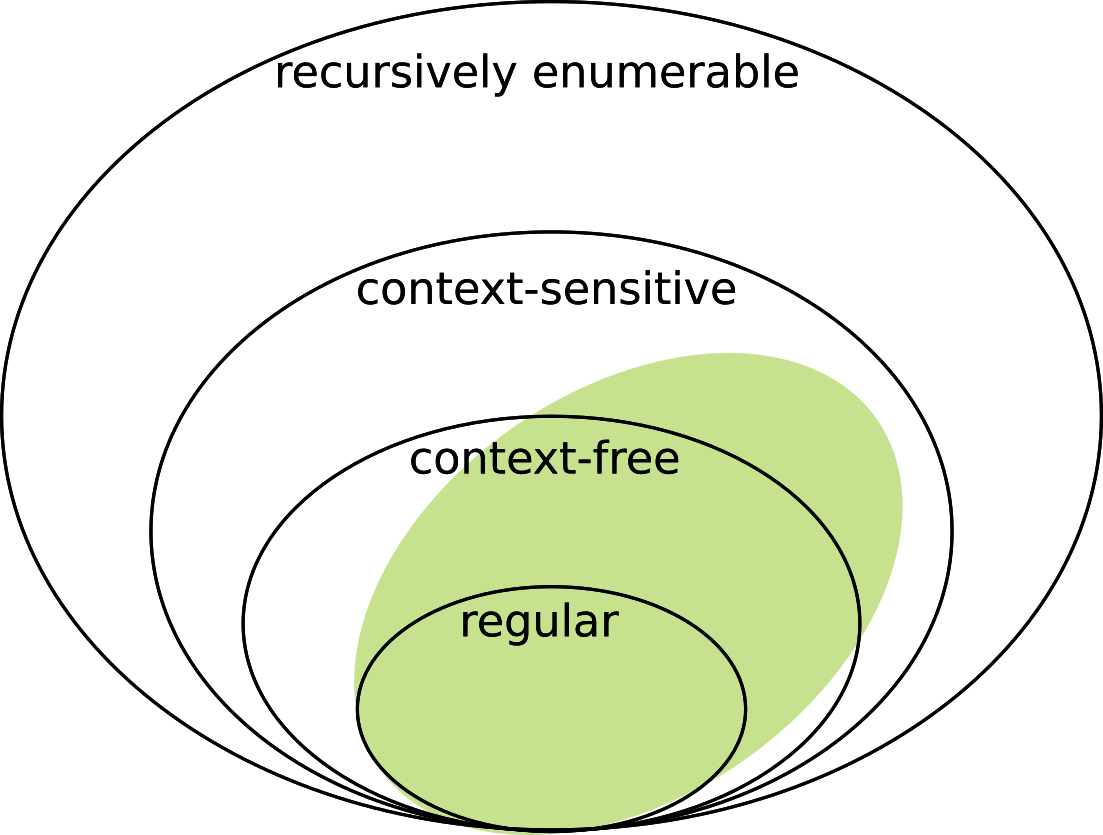
\includegraphics[width=0.4\linewidth]{chapters/chomsky}
  \caption{Lower bound on the expressivity of the subset of CG using only \t{REMOVE}.}
  \label{fig:nocorr}
\end{figure}

\subsection{A lower bound for CG}\label{sec:lowerbound}
In this section, we will only use the \t{REMOVE} command with sections, in
addition to a single use of the \t{ADDCOHORT} command to add the special cohort
\t{"<REJECT>"}, and a single use of the \t{REMCOHORT} command to clean up
afterwards. 
We show that, using only these commands, CG is capable of generating some
context-free and context-sensitive languages, which establishes a lower bound on 
the expressivity of CG (see Figure~\ref{fig:nocorr}).


\paragraph{Example grammar: $a^nb^n$}
Below, we briefly describe the CG which generates the language $a^nb^n$.
This CG is defined over the alphabet $\Sigma$, in addition to a hidden alphabet
$\Sigma^\prime$. These hidden symbols are meant to serve as a simple form of
memory. When we encode our input words, we tag each cohort with \emph{every}
symbol in the hidden alphabet\footnote{
  We can automatically add these hidden symbols to our cohorts using a single
  application of the \t{ADD} command.
}, e.g.\ for some symbol $\ell \in \Sigma$ and $\Sigma' = \{h_1,\dots,h_n\}$ we
would create the cohort \(\t{"<\(\ell\)>"}\;\t{"h\(_1\)"}\;\dots\;\t{"h\(_n\)"}\).

The CG for $a^nb^n$ uses the hidden alphabet \{\t{odd}, \t{even}, \t{opt\_a},
\t{opt\_b}\}. These symbols mean that the cohort they are attached to is in an
even or odd position, and that $a$ or $b$ is a legal option for this cohort,
respectively. The CG operates as follows: 
\begin{enumerate}
\item
  Is the number of characters even? We know the first cohort is odd, and the
  rest is handled with rules of the form \t{REMOVE even IF (NOT -1 odd)}. If the
  last cohort is odd, then discard the sentence. Otherwise continue\dots
\item
  The first cohort is certainly $a$ and last is certainly $b$, so we can
  disambiguate the edges: 
  \t{REMOVE opt\_b IF (NOT -1 (*))}, and \t{REMOVE opt\_a IF (NOT 1 (*))}. 
\item
  Disambiguate the second cohort as $a$ and second-to-last as $b$, the third as
  $a$ and third-to-last as $b$, etc, until the two ends meet in the middle. If
  every \t{"<a>"} is marked with \t{opt\_a}, and every \t{"<b>"} with
  \t{opt\_b}, we accept. Otherwise, we reject.  
\end{enumerate}
The language $a^nb^n$ is context-free, and therefore CG must at least partly
overlap with the context-free languages.


\paragraph{Example grammar: $a^nb^nc^n$}
We can extend the approach used in the previous grammar to write a grammar which
accepts $a^nb^nc^n$. Essentially, we can adapt the above grammar to find the
middle of any input string. Once we have the middle, we can ``grow'' $a$s from
the top and $b$s up from the middle, and $b$s down from the middle and $c$s up
from the bottom, until we divide the input into three even chunks.
If this ends with all \t{"<a>"}s marked with \t{opt\_a}, all \t{"<b>"}s marked
with \t{opt\_b}, and all \t{"<c>"}s marked with \t{opt\_c}, we accept.
Otherwise, we reject.

The language $a^nb^nc^n$ is context-sensitive, and therefore CG must at least
partly overlap with the context-sensitive languages.

\begin{figure}[h]
  \centering
  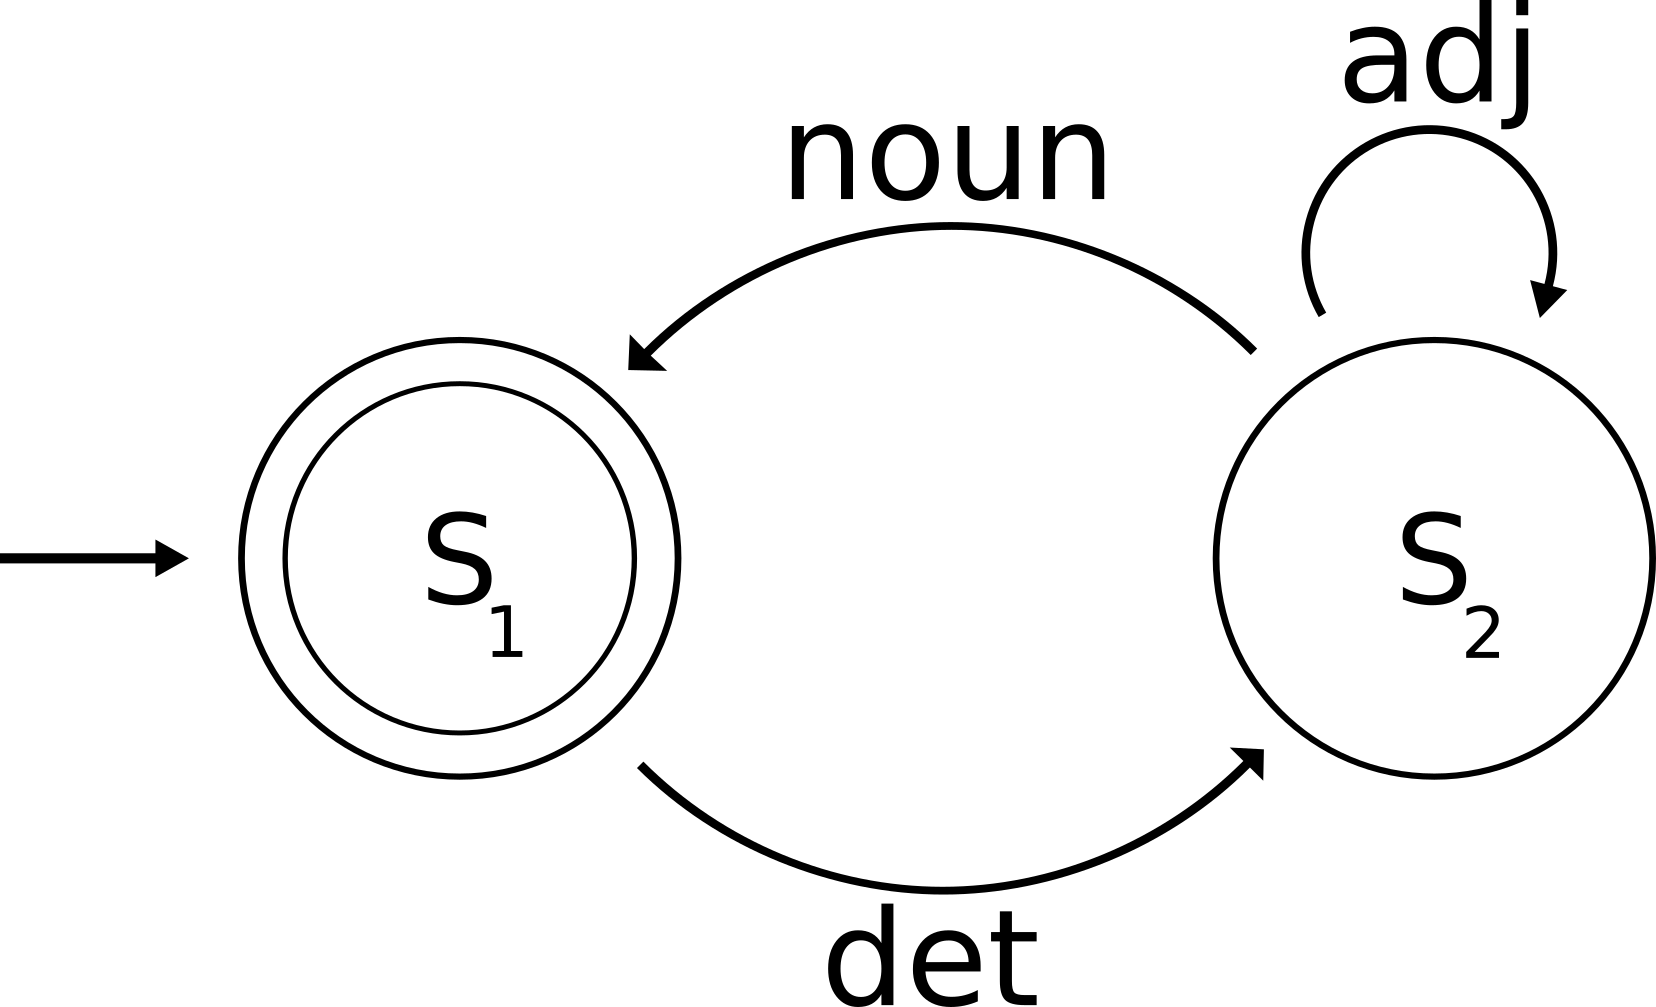
\includegraphics[width=0.4\linewidth]{chapters/fsa.png}
  \caption{A finite-state automaton describing the regular language \t{det
      (adj)* noun}.}
 \label{fig:fsa}
\end{figure}

\subsection{CG is regular}\label{sec:regular}
In the present section, we propose a method to transform arbitrary
finite-state automata into CG. We show how any finite-state automaton
can be expressed in a CG: encode the states and transitions as
ambiguous cohorts, and the disambiguated result shows both the correct
sequence and its path in the automaton.  The translation is
implemented in Haskell, and can be found on GitHub\footnote{See
  \url{https://github.com/inariksit/cgexp}}.



\paragraph{Finite-state automata}
Formally, a finite-state automaton is a 5-tuple
\[
  \langle \Sigma, S, s_0, \delta, F \rangle.
\]


\noindent $\Sigma$ is the alphabet of the automaton, $S$ is a set of states,
including a starting state $s_0$ and a set $F$ of final states.
$\delta$ is a transition function, which takes one state and one
symbol from the alphabet, and returns the state(s) where we can get
from the original state with that symbol.
The automaton in Figure~\ref{fig:fsa} is presented as follows:

\[\!
\begin{aligned}
  &S&      \!\!\!\!=\;& \{\t{s1}, \t{s2}\}  &&\Sigma& \!\!\!\!=\;& \{\emph{det, adj, n}\} \\
  &s_0&    \!\!\!\!=\;& \t{s1}              &&\delta& \!\!\!\!=\;& \{\t{s1} \xrightarrow{\text{\em det}} \{\t{s2}\},  \\ 
  &F&      \!\!\!\!=\;& \{\t{s1}\}          &&      & \!\!\!\! \;& \ \t{s2} \xrightarrow{\text{\em adj}} \{\t{s2}\}, \\
  & &                 &                     &&      & \!\!\!\! \;& \ \t{s2} \xrightarrow{\text{\em noun}} \{\t{s1}\} \} \\
\end{aligned}
\]

Informally, the automaton describes a simple set of possible noun
phrases: there must be one determiner, one noun, and 0 or more
adjectives in between. 
We implement a corresponding CG in the following sections.


\paragraph{Cohorts and sentences}

We encode our input as a sequence of \emph{state cohorts} and \emph{transition cohorts}.
Initially, a state cohort contains the full set $S = \{\t{s1}, \t{s2}\}$ as
its readings, and a transition cohort contains the alphabet $\Sigma =
\{\emph{det, adj, noun}\}$, or some subset of it. As an example, we
generate all 2-letter words recognised by the automaton in
Figure~\ref{fig:fsa}. The initial maximally ambiguous input for length
2 looks as follows:
%
\begin{center}
  \renewcommand{\tabcolsep}{2.5pt}
  \begin{tabular}{ccccc}
    \swf   & \t{"<w>"}  & \swf   & \t{"<w>"} & \swf   \\ 
    \h{s1} & \t{det}      & \h{s1} & \t{det} & \h{s1} \\
    \h{s2} & \t{adj}      & \h{s2} & \t{adj} & \h{s2} \\
           & \t{noun}     &        & \t{noun} &               
  \end{tabular}
\end{center}
%
\noindent 
The grammar disambiguates both transition cohorts and state cohorts. Thus
the desired result shows both the accepted sequence(s)---\emph{det noun}
in this case---and their path(s) in the automaton.
%
\begin{center}
  \renewcommand{\tabcolsep}{2.5pt}
  \begin{tabular}{ccccc}
    \swf   & \t{"<w>"}  & \swf   & \t{"<w>"} & \swf   \\ 
    \h{s1} & \t{det}    & \h{s2} & \t{noun}  & \h{s1}       
  \end{tabular}
\end{center}
%
We can easily adapt the disambiguation scheme for real-world
ambiguities, such as ``the \exampleWord{}''. The state cohorts are identical, but the transition
cohorts contain now some actual word form, and the initial ambiguity
is not over the whole $\Sigma$, but some subset of it.
%
\begin{center}
  \renewcommand{\tabcolsep}{2.5pt}
  \begin{tabular}{ccccc}
    \swf   & \t{"<the>"}  & \swf   & \t{"<\exampleWord{}>"} & \swf    \\ 
    \h{s1} & \t{det}      & \h{s1} & \t{adj}   & \h{s1}  \\
    \h{s2} &              & \h{s2} & \t{noun}  & \h{s2}     
  \end{tabular}
\end{center}
%
The disambiguation process goes exactly like in the first version, with full
$\Sigma$ in the transition cohorts.
Depending on how much the initial input contains ambiguity, the
result may be the same, or more disambiguated. For our example, the
output is identical.
\begin{center}
  \renewcommand{\tabcolsep}{2.5pt}
  \begin{tabular}{ccccc}
    \swf   & \t{"<the>"}  & \swf   & \t{"<\exampleWord{}>"} & \swf    \\ 
    \h{s1} & \t{det}      & \h{s2} & \t{noun} & \h{s1}  \\
  \end{tabular}
\end{center}
%
%
\paragraph{Rules}
Given that every transition happens between two states, and every state 
has an incoming and outgoing transition, every rule needs only
positions -1 and 1 in its contextual tests. 
The semantics of the rules are ``remove a transition, if it is 
\emph{not} surrounded by allowed states'',
and ``remove a state, if it is \emph{not} surrounded by allowed transitions''.
For the example automaton, the rules are as follows:

\begin{itemize}
\item[]
\begin{verbatim}
# Transition rules                          # State rules
REMOVE Det                                  REMOVE S1          
    IF (NEGATE -1 S1 LINK 2 S2) ;               IF (NEGATE -1 >>> OR Noun
REMOVE Adj                                             LINK 2 Det) ;
    IF (NEGATE -1 S2 LINK 2 S2) ;           REMOVE S2
REMOVE Noun                                     IF (NEGATE -1 Det OR Adj
    IF (NEGATE -1 S2 LINK 2 S1) ;                      LINK 2 Adj OR Noun) ;
\end{verbatim}

\end{itemize}



The start and end states naturally correspond to the first and last
state cohort, and can be trivially disambiguated, in this case both into \t{s1}.
Once we remove a reading from either side of a cohort, some more rules can take
action---the context ``\t{s2} on the left side and \t{s1} on the right side''
may be broken by removing either \t{s2} or \t{s1}. 
One by one, these rules disambiguate the input, removing impossible
states and transitions from the cohorts.



\noindent For the final result of the disambiguation, we consider three options:
the cohorts may contain the whole alphabet, a well-formed subset
or a malformed subset.

\paragraph{Full $\Sigma$}
If there is only one allowed word of length $n$ in the language,
then the result will contain only fully disambiguated transition
cohorts.
Furthermore, if there is only path in the automaton that leads
to this word, then also the state cohorts are fully disambiguated.

If there are multiple words of the same length in the language, then
we have to relax our criteria: every transition cohort and state
cohort in the result may contain multiple readings, but all of them
must contribute to some valid word of length $n$, and its path in the
automaton. 

\paragraph{Well-formed subset of $\Sigma$}
With well-formed subset, we mean that each cohort contains
at least one of the correct readings: \{\t{det}\} for ``the'', and
\{\t{adj,noun}\} for ``\exampleWord{}''. 
If the initial input is well-formed, then the result will be correct,
and may even be disambiguated further than with the full $\Sigma$ in
the transition cohorts.

\paragraph{Malformed subset of $\Sigma$}
Malformed subset has at least one cohort without any correct readings,
for example, ``the'' is missing a \t{det} reading.
This will lead to arbitrary disambiguations, which do not correspond to the automaton.
Without a \t{det} reading in ``the'', the rule which removes \t{s2}
would trigger in the middle state, leaving us with three \t{s1}
states. \t{s1-s1-s1} is an impossible path in the automaton,
so it would trigger all of the transition rules, and stop only when
there is one, arbitrary, reading left in the transition cohorts.



%Given that the lack of disjunction is a fundamental design of CG, we do not envision a way to work around this limitation. 

\subsection{Discussion}

%\paragraph{Limitations of the FSA$\rightarrow$CG conversion}
Another question is, even if we had a working conversion system for
CFGs, would the result be correct?
As \newcite{lager_nivre01} point out, CG has no way of expressing disjunction.
Unlike its close cousin FSIG \cite{koskenniemi90}, which would represent a 
language such as $\{ab,ba\}$ faithfully, CG substitutes uncertainty on the 
sentence level (``either $ab$ or $ba$'') with uncertainty in the cohorts: 
``the first character may be either $a$ or $b$, and the second character 
may be either $a$ or $b$''.
If we use such a CG to generate, by feeding it
maximally ambiguous cohorts, the result will be overly permissive.
We acknowledge that this is a limitation in the expressive power: many
languages can only be approximated by CG, not reproduced exactly.
Nevertheless, this limitation may not matter so much when
disambiguating real-world text, because the cohorts are initially less
ambiguous, and leaving genuine ambiguity intact is desired behaviour
for CG. 



\section{Conclusions and future work}

We set out to design and implement an automatic analysis of constraint grammars that can find problematic rules and rule combinations, without the need for a corpus.
Our evaluation indicates that the tool indeed finds non-trivial conflicts and dead rules
from actual grammars. 

We did not have a volunteer to test the tool in
the process of grammar writing, so we cannot conclude whether the
constructed examples are useful for getting new insights on the rules.
In any case, there are still a number of features to improve and add.
Future work can be divided in roughly three categories: 
\begin{inparaenum}
\item[(a)] general improvement of the tool
\item[(b)] evaluation with users, and 
\item[(c)] integration as a part of CG development framework.
\end{inparaenum}

\subsection{General improvement}

\paragraph{Combining morphological and lexical tags}

Our solution to hardcode the tag combinations in the readings is
feasible for simple morphology, but it can cause problems with more
complex morphology. Currently, if we add one new lemma to the set of
readings, we need to create as many new variables as there are
inflectional forms for that lemma.  The alternative scheme we
implemented for Basque resulted in fewer combinations, but as a
result, it created nonsensical combinations of wordform, lemma and
morphological tags. Investigating whether this is a problem (i.e. does
it miss actual conflicts, or suggest false positives) is left for
future work.


\paragraph{Heuristic checks for common issues} 
As mentioned earlier, some grammar design choices are common sources
of misinterpretation.  Many of these issues concern the case where the
conditions include the target cohort---does \t{SELECT foo IF (0 bar)}
mean that ``foo'' and ``bar'' should be in the same reading or in
different readings?  Lemmas and word forms are another source of
confusion, which is easy to check automatically against the lexicon.
Ideally, these checks should be included in a special ``paranoid
mode'', to not clutter the analysis\footnote{As pointed out by Eckhard
  Bick, the program should act upon this only if the 0 relates to an
  existing ambiguity class.}.


\paragraph{Support for more features of VISL CG-3}
As for longer-term goals, we want to handle more of the features in
VISL CG-3, such as \textsc{map}, \textsc{append} and
\textsc{substitute} rules, as well as dependency structure.  This also
means finding different kinds of conflicts, such as dependency
circularity.  In order to implement rules that may add new readings,
or new tags to existing readings, we need to modify our approach in
the SAT-encoding.  Even if the lexicon gives all readings that exist
in the lexicon, the user might give a nonexistent reading, or in the
case of {\sc map}, a syntactic tag, which is (by definition) not in
the lexicon. We may need to move to a more scalable solution.

\subsection{Evaluation with user base}

Cleaning up the Basque grammar was our first chance to test the tool
together with grammarians, complemented with machine learning (the
tuning step). We got to a promising start, but due to the performance
problems, we had to simplify our approach considerably. Below, we
envision some properties that might be interesting to test further;
however, we would be interested in getting feedback from actual
grammarians and adding features based on what is needed.

\paragraph{Reformatting a rule}

Another possible feature is to suggest reformattings for a rule. Recall
Figure~\ref{fig:infrules} from the introduction; in the case on the right, the
original rule was written by the original author, and another
grammarian thought that the latter form is nicer to read. Doing the
reverse operation could also be possible. If a rule with long
disjunctions conflicts, it may be useful to split it into smaller
conditions, and eliminate one at a time, in order to find the
reason(s) for the conflict.


\paragraph{Suggesting alternative orders} 
On a speculative note, it could be interesting to identify pairs for a
potential ``feeding order'' that is missed in the grammar. Say we have
the following rule sequence:

\begin{itemize}
\item[]
\begin{verbatim}
REMOVE:r1 x IF (-1C y)
SELECT:s2 y IF (...)
\end{verbatim}
\end{itemize}

If $s2$ appears before $r1$, if makes way for $r1$ to act later on the
same round.  However, if the rules are ordered as shown, and $y$ is
not unambiguous from the beginning, then $r1$ has to wait for the next
round to be applied.

Lager \cite{lager01transformation} observed that the rule sequence
learned by the $\mu$TBL system did not remove further ambiguities
after its first run, and concluded that the sequence was ``optimal''.
It would be interesting to recreate the goals in
\cite{lager01transformation} and \cite{bick2013tuning}, to see if this
semantic analysis of rule dependencies could lead also to better
ordering within a grammar.

Of course, it remains to be seen if any of these improvements would
make a difference in speed; VISL CG-3 is already very fast, when the
grammars are run multiple times.

\paragraph{Alternative ways of deriving CGs}

Learning CG rules from a corpus has been a popular topic since the
beginning of the formalism
\cite{inducing_cg1996,lindberg_eineborg98ilp,lager01transformation,asfrent14}.
As an alternative, our method of transforming regular grammars into an
approximate CG (see Section~\ref{sec:expressivity} could be of
interest. To be fair, the resulting grammars are not very readable:
they include extra cohorts and symbols, and the logic is spread across
rules in a rather obscure way---in contrast to a human-written
grammar, where each rule is a self-contained piece of truth about a
language.  Therefore we do not envision the generated grammars being
used as is, but rather as compilation targets.  Such CGs could be used
as a part of a larger constraint grammar: some sections can be written
manually, and others derived from existing grammars. So far we only
have a working conversion tool for finite-state automata, but we are
hoping to develop this further, to also include context-free or even
mildly context-sensitive grammars.


\subsection{Integration as a part of CG development environment}

In order to attract the attention of the CG community, it would be
desirable to incorporate the tools as a part of existing CG software.
Currently, the described software consists of just under 3000 lines of
Haskell code, including both the CG engine and the grammar analysis
tool.  The grammar used for parsing the original CG files is written
in BNFC \cite{bnfc}, and it is missing many constructs in CG-3.  Given
these factors, the preferred option would be a full reimplementation
and integration as a part of VISL CG-3, or any other CG development
framework. We believe this would make the tools easier to use, more
cohesive and synchronised with the main CG engine, and likely much
faster. Of course, it is up to the community and the developers to
decide if these tools are of interest.
